\documentclass[a4paper,leqno]{amsart}
\usepackage[margin=30truemm]{geometry}
\usepackage{fancyhdr,appendix,graphicx,layout}
%\usepackage{stix2}
\usepackage{amsmath,amsthm,amssymb}
\usepackage[shortlabels]{enumitem}
\setlist[enumerate]{font=\normalfont}
\usepackage{physics}

\usepackage[numbers]{natbib}
\usepackage{bbm}
\usepackage{bm}
\usepackage{tikz}
\usepackage{tikz-cd}
\usetikzlibrary{positioning,arrows.meta,decorations.markings,calc}
\tikzset{
    cells={font=\everymath\expandafter{\the\everymath\displaystyle}},
}
\usepackage{caption}
\usepackage[pagewise]{lineno}

\usepackage{float}

\usepackage{color}
\definecolor{darkgreen}{rgb}{0,0.7,0}
\newcommand{\comment}[1]{{\color{darkgreen}#1}}
\definecolor{darkblue}{rgb}{0,0,0.7} % darkblue color
\newcommand{\defn}[1]{\textsl{\color{darkblue} #1}}
\newcommand{\old}[1]{{\color[rgb]{1,0,0}#1}}
\newcommand{\new}[1]{{\color[rgb]{0,0,1}#1}}
\newcommand{\bhx}[1]{{\color[rgb]{0.9,0.7,0.2}#1}}

%\renewcommand{\emph}[1]{\textcolor{blue}{\textit{#1}}}

\usepackage[hyperpageref]{backref}
\usepackage[pagebackref]{hyperref}
\hypersetup{
    colorlinks=true,
    linkcolor=red,  %section,table of contents
    filecolor=blue,  %local file link
    urlcolor=orange, %url
    citecolor=violet   %citation
}
\renewcommand*{\backref}[1]{}  
   \renewcommand*{\backrefalt}[4]{
      \ifcase #1 
         Not cited.
      \or
         Cited on page #2.
      \else
         Cited on pages #2.
      \fi}

\usepackage{cleveref}
\newcommand{\hyt}[1]{\hypertarget{#1}{\textit{\textcolor{Blue}{#1}}}}
\newcommand{\hyl}[1]{\hyperlink{#1}{#1}}

%%%%%%%%%%%%%%%%%%%%%%%%%%%%%%%%%%%%%%%%%%%%%%%%%
\makeatletter
\newcommand\ReDeclareMathOperator[2]{%
    \begingroup \escapechar\m@ne\xdef\@gtempa{{\string#1}}\endgroup
    \expandafter\@ifundefined\@gtempa
        {\@latex@error{Command \string#1 undefined}\@ehc}
        \relax
    \let\@ifdefinable\@rc@ifdefinable
    \DeclareMathOperator#1{#2}}
\makeatother

%%%%%%%%%%%%%%%%%%%%%%%%%%%%%%%%%%%%%%%%%%%%%%%%%%%%

% Crefname
\crefname{thm}{Theorem}{Theorems}
\crefname{dfn}{Definition}{Definitions}
\crefname{dfnprop}{Definition-Proposition}{Definition-Proposition}
\crefname{prop}{Proposition}{Propositions}
\crefname{lem}{Lemma}{Lemmas}
\crefname{cor}{Corollary}{Corollaries}
\crefname{clm}{Claim}{Claims}
\crefname{ass}{Assumption}{Assumption}
\crefname{cond}{Condition}{Condition}
\crefname{nota}{Notation}{Notation}
\crefname{conj}{Conjecture}{Conjecture}
\crefname{fct}{Fact}{Facts}
\crefname{rmk}{Remark}{Remarks}
\crefname{eg}{Example}{Examples}
\crefname{que}{Question}{Questions}
\crefname{figure}{Figure}{Figures}
\crefname{table}{Table}{Tables}
\crefname{section}{Section}{Sections}
\crefname{subsection}{Subsection}{Subsections}
\crefname{appendix}{Appendix}{Appendices}
\crefname{equation}{}{}
\crefname{main}{Theorem}{Theorems}

% Theoremstyle
\theoremstyle{plain}
\newtheorem{thm}{Theorem}[section]
\newtheorem{main}{Theorem}
\newtheorem{prop}[thm]{Proposition}
\newtheorem{lem}[thm]{Lemma}
\newtheorem{cor}[thm]{Corollary}

\theoremstyle{definition}
\newtheorem{dfn}[thm]{Definition}
\newtheorem{dfnprop}[thm]{Definition-Proposition}
\newtheorem{dfnlem}[thm]{Definition-Lemma}
\newtheorem{clm}[thm]{Claim}
\newtheorem{ass}[thm]{Assumption}
\newtheorem{cond}[thm]{Condition}
\newtheorem{nota}[thm]{Notation}
\newtheorem{conj}[thm]{Conjecture}
\newtheorem{fct}[thm]{Fact}
\newtheorem{eg}[thm]{Example}
\newtheorem{que}[thm]{Question}

\theoremstyle{remark}
\newtheorem{rmk}[thm]{Remark}
\numberwithin{equation}{section}
\makeatletter
\let\c@equation\c@thm
\makeatother
\renewcommand{\themain}{\Alph{main}}

% Letter
\newcommand{\A}{\mathcal A}
\newcommand{\D}{\mathcal D}
\renewcommand{\H}{\mathcal H}
\newcommand{\T}{\mathcal T}
\newcommand{\U}{\mathcal U}
\newcommand{\V}{\mathcal V}
\newcommand{\W}{\mathcal W}

\newcommand{\RR}{\mathbf{R}}
\newcommand{\LL}{\mathbf{L}}

\newcommand{\NN}{\mathbb N}
\newcommand{\ZZ}{\mathbb{Z}}


%Arrow
\newcommand{\mono}{\hookrightarrow}
\newcommand{\epi}{\twoheadrightarrow}
\newcommand{\iso}{\similarrightarrow}
\newcommand{\xto}{\xrightarrow}
\newcommand{\LR}{\Leftrightarrow}
\newcommand{\To}{\Rightarrow}


% Abelian Category
\DeclareMathOperator{\Fac}{Fac}
\DeclareMathOperator{\Sub}{Sub}
\DeclareMathOperator{\Filt}{Filt}
\DeclareMathOperator{\add}{add}
\DeclareMathOperator{\Add}{Add}
\DeclareMathOperator{\rad}{rad}
\ReDeclareMathOperator{\top}{top}
\DeclareMathOperator{\simp}{Sim}
\DeclareMathOperator{\id}{id}
\DeclareMathOperator{\ind}{ind}
\DeclareMathOperator{\cok}{cok}
\DeclareMathOperator{\proj}{proj}
\DeclareMathOperator{\inj}{inj}
\DeclareMathOperator{\colim}{colim}
\DeclareMathOperator{\obj}{obj}
\DeclareMathOperator{\Mod}{\mathcal Mod}
\let\mod\relax
\DeclareMathOperator{\mod}{mod}
\DeclareMathOperator{\fl}{fl}
\DeclareMathOperator{\grmod}{grmod}
\DeclareMathOperator{\Grmod}{Grmod}
\DeclareMathOperator{\sdim}{\st{dim}}



%Triangulated category
\DeclareMathOperator{\thick}{thick}
\DeclareMathOperator{\cone}{cone}
\DeclareMathOperator{\per}{per}
\DeclareMathOperator{\pvd}{pvd}


%Functor
\DeclareMathOperator{\Hom}{Hom}
\DeclareMathOperator{\End}{End}
\DeclareMathOperator{\Aut}{Aut}
\DeclareMathOperator{\RHom}{\RR Hom}
\DeclareMathOperator{\REnd}{\RR End}
\DeclareMathOperator*{\ten}{\otimes}
\DeclareMathOperator*{\Ltensor}{\otimes^{\LL}}
\DeclareMathOperator{\Tot}{Tot}
\DeclareMathOperator{\Ext}{Ext}
\DeclareMathOperator{\Tor}{Tor}


% Non-crossing partition
\DeclareMathOperator{\NC}{NC}
\DeclareMathOperator{\wide}{wide}
\DeclareMathOperator{\Kr}{Kr}
\DeclareMathOperator{\cox}{cox}
\ReDeclareMathOperator{\l}{\ell}
\newcommand{\ora}{\overrightarrow}

% Others
\newcommand{\st}[1]{\underline{#1}}
\newcommand{\ts}[1]{\overline{#1}}
\DeclareMathOperator{\la}{\langle}
\DeclareMathOperator{\ra}{\rangle}
\newcommand{\wt}{\widetilde}

\newcommand{\val}{\operatorname{val}}
\newcommand{\Max}{\operatorname{Max}}
\newcommand{\Ker}{\operatorname{Ker}}
\newcommand{\Image}{\operatorname{Im}}
\newcommand{\vv}{\mathsf{v}}
\newcommand{\ww}{\mathsf{w}}

\newcommand{\BOne}{\left(\begin{smallmatrix} 1&0\\ 0&0\\ 0&0 \end{smallmatrix}\right)}
\newcommand{\AOne}{\left(\begin{smallmatrix} 0&0&0\\ 0&0&1 \end{smallmatrix}\right)}

\newcommand{\BTwo}{\left(\begin{smallmatrix} 0&0\\ 0&0\\ 1&0 \end{smallmatrix}\right)}
\newcommand{\ATwo}{\left(\begin{smallmatrix} 0&0&0\\ 1&0&0 \end{smallmatrix}\right)}

\newcommand{\BThree}{\left(\begin{smallmatrix} 1&0\\ 1&0\\ 1&0 \end{smallmatrix}\right)}
\newcommand{\AThree}{\left(\begin{smallmatrix} 0&0&0\\ -\lambda&1&\lambda-1 \end{smallmatrix}\right)}

\newcommand{\BOneN}{%
\left(\begin{smallmatrix}
I_n&0\\
0&0\\
0&0
\end{smallmatrix}\right)}

\newcommand{\AOneN}{%
\left(\begin{smallmatrix}
0&0&0\\
0&0&I_n
\end{smallmatrix}\right)}

\newcommand{\BTwoN}{%
\left(\begin{smallmatrix}
0&0\\
0&0\\
I_n&0
\end{smallmatrix}\right)}

\newcommand{\ATwoN}{%
\left(\begin{smallmatrix}
0&0&0\\
I_n&0&0
\end{smallmatrix}\right)}

\newcommand{\BThreeN}{%
\left(\begin{smallmatrix}
I_n&0\\
I_n&0\\
I_n&0
\end{smallmatrix}\right)}

\newcommand{\AThreeN}{%
\left(\begin{smallmatrix}
0&0&0\\
-J_n&I_n&J_n-I_n
\end{smallmatrix}\right)}

\newcommand{\morsethickarrow}{%
  \mathrel{\tikz[baseline=-0.55ex]
    \draw[->] (0,0) -- (1.6em,0);}}
\newcommand{\morsedottedarrow}{%
  \mathrel{\tikz[baseline=-0.55ex]
    \draw[densely dotted,line cap=round,->]
    (0,0) -- (1.6em,0);}}

\DeclareMathOperator{\domdim}{domdim}
\DeclareMathOperator{\fdim}{fdim}
\DeclareMathOperator{\idim}{idim}
\DeclareMathOperator{\pdim}{pdim}
\DeclareMathOperator{\gldim}{gldim}
\DeclareMathOperator{\supp}{supp}
\DeclareMathOperator{\Crit}{Crit}
\DeclareMathOperator{\Ind}{Ind}
\DeclareMathOperator{\sd}{sd}
\DeclareMathOperator{\weight}{wt}
\DeclareMathOperator{\diam}{diam}
\newcommand{\SDiff}{\mathbin{\triangle}}
\DeclareMathOperator{\MH}{MH}
\DeclareMathOperator{\lat}{lat}


\title[Gorenstein distance algebras of lattices]{Distance algebras of finite distributive lattices are Gorenstein}
\author{Aaron Chan and Bohan Xing}
\date{\today}

\newcommand{\Addresses}{{% additional braces for segregating \footnotesize
  \bigskip
  \footnotesize

  A. Chan, \textsc{Department of mathematics, Nagoya University, Chikusa-ku, Nagoya 464-8602, Japan}\par\nopagebreak
  \textit{E-mail address}: \texttt{aaron.kychan@gmail.com}

  \medskip

  B. Xing, \textsc{School of Mathematical Sciences, Laboratory of Mathematics and Complex Systems, Beijing Normal University, Beijing 100875, P.R. China}\par\nopagebreak
  \textit{E-mail address}: \texttt{bhxing@mail.bnu.edu.cn}
}}

\begin{document}
\begin{abstract}
Let $L$ be a finite distributive lattice and let $\Sigma_L$ be the distance algebra of its Hasse graph.  For every indecomposable injective $\Sigma_L$-module, we construct a projective resolution  and use algebraic Morse theory to obtain a minimal resolution whose multiplicities are reduced Betti numbers of strict upset order complexes.  As a consequence, $\Sigma_L$ is (Iwanaga--)Gorenstein, with both self-injective dimensions bounded by the diameter of the Hasse graph of $L$.  We further prove that the first two terms of each minimal resolution are multiplicity-free, whereas arbitrary multiplicities occur in every higher projective degree.
\end{abstract}
\maketitle
\tableofcontents

\section{Introduction}
\label{sec:introduction}

Magnitude homology was introduced by Hepworth and Willerton as a categorification of the magnitude of a graph~\cite{HW17}. Its connection with homological algebra was made explicit by Asao and Ivanov, who realized magnitude homology as a derived functor over the distance algebra~\cite{AI24}. Asao and Wakatsuki subsequently constructed minimal projective resolutions for the distance algebras of geodetic metric spaces~\cite{AW24}. In this paper we study the distance algebras associated with the Hasse graphs of finite distributive lattices, a family in which shortest paths are generally not unique.

In our companion paper~\cite{CX26}, we studies broader representation-theoretic and homological properties of distance algebras of finite graphs. In particular, it shows that the distance algebra of a finite modular lattice is Auslander--Gorenstein precisely when the lattice is a finite direct product of chains. For a distributive lattice $L=\mathcal J(P)$, this is equivalent to every connected component of $P$ being a chain. The present paper establishes the Gorenstein and Iwanaga--Gorenstein properties for distance algebras of arbitrary finite distributive lattices under the corresponding assumptions on the coefficient ring.

By Birkhoff's fundamental theorem of distributive lattices, every finite distributive lattice has the form $L=\mathcal J(P)$ for a finite poset $P$. For the distance algebra $\Sigma_L$ over a commutative noetherian ring $R$, we construct a projective resolution of each module $I_X=D(\Sigma_L e_X)$, indexed by strict chains in a symmetric-difference poset. These resolutions have length at most $|P|=\diam(L)$, where $\diam(L)$ denotes the diameter of the Hasse graph of $L$. Together with the Gorenstein criterion of Iyengar--Krause~\cite[Theorem~4.6]{IK22}, this gives our first main result.

\begin{main}\label{main:minimal-resolution-and-ig}\textnormal{(see Corollary~\ref{cor:distributive-ig})}
Let $R$ be a commutative noetherian ring and let $L$ be a finite distributive lattice. Let $\Sigma_L$ be the distance $R$-algebra of its Hasse graph.
\begin{enumerate}
\item If $R$ is Gorenstein, then $\Sigma_L$ is a Gorenstein $R$-algebra.
\item If $R$ is Iwanaga--Gorenstein, then $\Sigma_L$ is Iwanaga--Gorenstein and
\[
 \idim (\Sigma_L)_{\Sigma_L}
 =\idim {}_{\Sigma_L}\Sigma_L
 \leq\diam(L)+\idim_R R.
\]
\end{enumerate}
\end{main}

Over a field $R=\Bbbk$, we use algebraic Morse theory~\cite{CLZ26} to obtain minimal projective resolutions of the indecomposable injectives. Their multiplicities and lengths are given by the reduced homology of the strict upset order complexes from Subsection~\ref{subsec:strict-upsets}; see Theorem~\ref{thm:minimal-resolution} and Corollary~\ref{cor:SigmaJ(P) is IG}. This also computes the self-injective dimension of $\Sigma_L$.

The combinatorics of order ideals forces multiplicity-freeness in the first two terms. For higher degrees, height-two posets identify the relevant order complexes with barycentric subdivisions of independence complexes of bipartite graphs. A realization theorem of Nagel and Reiner~\cite{NR09} then produces arbitrary multiplicities.

\begin{main}\label{main:minimal-resolution-and-multiplicities}\textnormal{(see Theorem~\ref{thm:minimal-resolution}, Proposition~\ref{prop:low-degree-multiplicity}, and Corollary~\ref{cor:arbitrary-higher-multiplicities})}
For every finite poset $P$ and every $X\in\mathcal J(P)$, we construct a minimal projective resolution of the indecomposable injective corresponding to $X$. These resolutions have the following properties.
\begin{enumerate}
\item The first two terms are multiplicity-free.
\item Multiplicities can be arbitrarily large in every higher projective degree.
\end{enumerate}
\end{main}

\medskip
\noindent
\textbf{Organization of the paper.} Section~\ref{sec:preliminaries} recalls distance algebras, Gorenstein algebras, distributive lattices, and order complexes of strict upsets. Section~\ref{sec:candidate-resolution} constructs the strict-chain projective resolutions, proves their exactness, and establishes Theorem~\ref{main:minimal-resolution-and-ig}. Section~\ref{sec:minimal-morse} uses algebraic Morse theory to construct the minimal resolutions and compute their lengths. Sections~\ref{sec:low-degree-multiplicity} proves Theorem~\ref{main:minimal-resolution-and-multiplicities}. Appendix~\ref{app:thin-modules} places the strict chain construction in a more general framework for thin modules over arbitrary finite-dimensional algebras.


\medskip
\noindent
{\bf Conventions and notation.}
Throughout, $R$ denotes a commutative noetherian ring with identity, and $\Bbbk$ denotes a field. All algebras are associative and unital. By an $R$-algebra we mean one that is finitely generated and projective as an $R$-module. Unless otherwise stated, modules are finitely generated right modules that are free over $R$. 
Unadorned tensor $\otimes$ between modules are tensor $\otimes_R$ over the ground ring $R$.
All graphs, posets, lattices, and simplicial complexes are finite. The symbols $\idim$ and $\pdim$ denote injective and projective dimension, respectively. We write $D:=\Hom_R(-,R)$; when the coefficient ring is specialized to $R=\Bbbk$, this means $D=\Hom_{\Bbbk}(-,\Bbbk)$. 

\medskip
\noindent
\textbf{Use of AI.}
The candidate complex is suggested to us by ChatGPT model 5.6 Sol, after we calculated the projective cover of the first syzygy (see subsection \ref{subsec:multi-free deg 0 1}); the appendix records our retrospect explanation in why one should consider such construction of complex. 
ChatGPT also suggested the strategy to show is exactness, helped us to refine the Morse matching described in Subsection~\ref{subsec:construction-morse-matching}, the entire subsection~\ref{subsec:higher-multiplicities}, and some of the figures throughout this notes.
All mathematical arguments were independently verified and finalized by the authors. The authors take full responsibility for the accuracy, originality, and integrity of the paper.

\medskip
\noindent
\textbf{Acknowledgements.}
%We thank Osamu Iyama for telling us about the connection between distance algeberas and tiled orders.  AC is deeply grateful for Yasuhiko Asao and Shun Wakatsuki on teaching him about the connection between distance algebras and magnitude homolgies, and the many discussions on the subject.
AC is supported by JSPS Grant-in-Aid for Scientific Research (C) 24K06666. BX is supported by the China Scholarship Council (No. 202506040127).

%%%%%%%%%%%%%%%%%%%%%%%%%%%%%%%%%%%%%%%%%%%%%%%%%%%%%%%%%%%%%
%%%%%%%%%%%%%%%%%%%%%%%%%%%%%%%%%%%%%%%%%%%%%%%%%%%%%%%%%%%%%

\section{Preliminaries}
\label{sec:preliminaries}

\subsection{Distance algebra}

Let $G=(V,E)$ be a connected combinatorial graph, where $V$ is the set of vertices and $E$ is the set of edges. In this paper, we assume that $G$ contains neither loops nor multiple edges.

For vertices $x,y\in V$, we write $\{x,y\}\in E$ if $x$ and $y$ are connected by an edge; in this case, they are called \defn{adjacent}. The \defn{distance} between $x$ and $y$, denoted by $$d(x,y)=d_G(x,y),$$ is the length of a shortest path from $x$ to $y$ on $G$, and the \defn{diameter} of $G$ is the maximal distance in $G$, denoted by $$\operatorname{diam}(G) :=\max_{x,y\in V}d(x,y).$$

\begin{dfn}
Let $G=(V,E)$ be a graph (without multi-edge and loops), and $Q_G$ be its \defn{double quiver}, i.e. the set of vertices of $Q_G$ is $V$ and there is a pair of arrows
\[\begin{tikzcd}
	x \arrow[r, "{a_{xy}}", bend left] & y \arrow[l, "{a_{yx}}", bend left]
\end{tikzcd} \text{ for each edge }\{x,y\}\in E.\]
The \defn{distance $R$-algebra} of $G$ is defined to be $\Sigma_G:=R Q_G/I_G$, where $I_G$ is the ideal generated by the following relations:
\begin{enumerate}
    \item $p=0$, for every path $p$ such that $\ell(p)>d(s(p),t(p))$;
    \item $p=q$, for every pair of paths $p,q$ in $Q_G$ with
$$s(p)=s(q),\qquad t(p)=t(q),\qquad
\ell(p)=d(s(p),t(p))=\ell(q).$$
\end{enumerate}
\end{dfn}

By definition, in $\Sigma_G$, a path is non-zero if and only if it is represented by a shortest path in $G$, and any two shortest paths with the same starting and ending vertices are identified. Hence, for any two vertices $x,y\in V$, there is a unique non-zero path from $x$ to $y$ modulo $I_G$. In particular, $e_x\Sigma_Ge_y$ is a free $R$-module of rank one for all $x,y\in V$, and $\Sigma_G$ is free of rank $|V|^2$ over $R$. When $R=\Bbbk$, the algebra $\Sigma_G$ is Schurian.


We take an $R$-basis $\{b_{xy}\mid x,y\in V\}$ for $\Sigma_G$, where $b_{xy}$ denotes the equivalence class of any shortest path from $x$ to $y$ on $G$, with the convention that $b_{xx}=e_x$ is the vertex idempotent associated to $x$. Then multiplication in $\Sigma_G$ is given by
$$
b_{xy}b_{yz}=
\begin{cases}
b_{xz}, & \text{if } d(x,z)=d(x,y)+d(y,z),\\
0, & \text{otherwise}.
\end{cases}
$$
Note that $b_{xy}$ is denoted by $(x,y)$ and by $e_{xy}$ in \cite{AI24} and \cite{AW24} respectively. Thus, each $\Sigma_G$ is an $R$-algebra.

Note that path length induces a natural grading on $\Sigma_G$; this matches the canonical (internal $\mathbb{R}$-)grading of magnitude homology.  Moreover, the assignment $b_{xy}\longmapsto b_{yx}$ defines an involutive anti-automorphism of $\Sigma_G$. Consequently, it induces an isomorphism of algebras $\Sigma_G^{\operatorname{op}}\cong\Sigma_G$.

The graphs that we concern in this note are the Hasse diagrams of finite distributive lattices $L$.  We will simplify the notation and write $\Sigma_L$.


%%%%%%%%%%%%%%%%%%%%%%%%%%%%%%%%%%%%%%%%%%%%%%%%%%%%%%%%%%

\subsection{Duality and Gorenstein algebras}
\label{subsec:duality-gorenstein}

Let $A$ be a finite projective $R$-algebra.

Recall that a ring $B$ is \defn{Iwanaga--Gorenstein} if it is noetherian on both sides and
\[
 \idim B_B<\infty
 \qquad\text{and}\qquad
 \idim {}_B B<\infty.
\]
A finite projective $R$-algebra $A$ is called a \defn{Gorenstein $R$-algebra} if $A_{\mathfrak p}$ is Iwanaga--Gorenstein for every $\mathfrak p\in\operatorname{Spec}R$ such that $A_{\mathfrak p}\neq0$; see \cite[Definition~1.1]{IK22} and \cite[Definition~6.1]{GIK23}. When $R=\Bbbk$, this is precisely the Iwanaga--Gorenstein property.

Following Buchweitz \cite[Section~7.6]{Buc21}, we call
\[
 \omega_{A/R}:=D(A),
 \qquad
 (a f b)(c):=f(bca)
 \quad(a,b,c\in A,\ f\in D(A)).
\]
the \defn{dualizing bimodule} of $A$.
When $R$ is Gorenstein, a criterion of Iyengar--Krause states that $A$ is a Gorenstein $R$-algebra if and only if
\begin{equation}
 \pdim_A(\omega_{A/R})<\infty
 \qquad\text{and}\qquad
 \pdim_{A^{\operatorname{op}}}(\omega_{A/R})<\infty;
 \label{eq:canonical-finite-pdim}
\end{equation}
equivalently, $\omega_{A/R}$ admits a bounded resolution by finitely generated projective modules on each side; see \cite[Theorem~4.6]{IK22} or \cite[Theorem~6.7]{GIK23}.  For the distance algebras of finite distributive lattices, we will prove condition \eqref{eq:canonical-finite-pdim} without assuming that $R$ is Gorenstein.  When $R$ is Gorenstein, the above criterion then shows that these are Gorenstein $R$-algebras.

An \defn{$A$-lattice} is a right $A$-module whose underlying $R$-module is finitely generated and projective. We write $\lat(A)$ for the category of $A$-lattices, equipped with the exact structure inherited from the category of $A$-modules. Every short exact sequence in this category splits over $R$.

\begin{lem}\textnormal{(cf. \cite[Section~1]{Rum04})}\label{lem:lattice-canonical-duality}
The functor $D$ induces an exact duality
\[
 D:\lat(A)^{\operatorname{op}}
 \xrightarrow{\sim}\lat(A^{\operatorname{op}}).
\]
The category $\lat(A)$ has enough projective and injective objects, given by $\add A$ and $\add\omega_{A/R}$, respectively. Moreover, the projective dimension of an $A$-lattice in $\lat(A)$ equals its ordinary projective dimension.
\end{lem}

\begin{proof}
The functor $D$ is exact on $R$-split short exact sequences, and evaluation gives a natural isomorphism $M\xrightarrow{\sim}D^2(M)$ for every $M\in\lat(A)$. This proves the duality assertion.

For $M\in\lat(A)$, choose a surjection $A^m\twoheadrightarrow M$ with $m$ finite. It splits over $R$, so its kernel is again an $A$-lattice. Thus $\lat(A)$ has enough projectives, and its projective objects are precisely $\add A$. Applying the duality to the corresponding assertion for left modules gives the assertion about injectives. Repeating the construction produces a resolution by finitely generated projective $A$-modules with lattice syzygies. If the ordinary projective dimension is finite, the syzygy in that degree is projective, proving the last assertion.
\end{proof}

We call the objects of $\add\omega_{A/R}$ \defn{relative injective} $A$-modules. For $M\in\lat(A)$, write $\operatorname{relidim}_A M$ for its relative injective dimension in $\lat(A)$, namely, the least length of a coresolution by relative injectives, or $\infty$ if no finite such coresolution exists. When $R=\Bbbk$, relative injectives are the finitely generated ordinary injectives, and relative injective dimension agrees with ordinary injective dimension.

We now consider the distance algebra $\Sigma_G$ of a finite connected graph $G$ over $R$. The basis $\{b_{xy}\mid x,y\in V(G)\}$ makes $\Sigma_G$ a finite free $R$-module. For $x\in V(G)$, set
\[
 P_x:=e_x\Sigma_G,
 \qquad
 I_x:=D(\Sigma_G e_x).
\]
These are projective and relative injective right $\Sigma_G$-modules, respectively, and
\[
 (\Sigma_G)_{\Sigma_G}=\bigoplus_{x\in V(G)}P_x,
 \qquad
 (\omega_{\Sigma_G/R})_{\Sigma_G}=\bigoplus_{x\in V(G)}I_x.
\]
When $R=\Bbbk$, $P_x$ and $I_x$ are indecomposable, and $I_x$ is the injective envelope of $S_x:=P_x/\rad P_x$.

Path reversal defines an $R$-linear anti-involution
\[
 \tau:\Sigma_G\longrightarrow \Sigma_G,
 \qquad b_{xy}\longmapsto b_{yx}.
\]
For a right $\Sigma_G$-module $M$, let $\tau_*M$ be the left $\Sigma_G$-module with action $a\cdot m:=m\tau(a)$. This gives a covariant exact equivalence between right and left module categories, preserving projectives and injectives. Its inverse is defined by the same construction for left modules. Since $\tau(e_x)=e_x$, there is an isomorphism of left $\Sigma_G$-modules
\begin{equation}
 \tau_*I_x\xrightarrow{\sim}D(e_x\Sigma_G),
 \qquad f\longmapsto\bigl(b\longmapsto f(\tau(b))\bigr).
 \label{eq:tau-canonical-summands}
\end{equation}
Thus, we have the following lattice version of duality on distance algebras \cite[Section~2]{CX26}.  

\begin{prop}\label{prop:distance-lattice-duality}
For $M\in\lat(\Sigma_G)$, equip $D(M)$ with the right $\Sigma_G$-action
\[
 (f\cdot a)(m):=f\bigl(m\tau(a)\bigr).
\]
With this right action, $D$ defines an exact contravariant self-duality of $\lat(\Sigma_G)$, with $ D(P_x)\cong I_x$ and $D(I_x)\cong P_x$. Consequently, for every $M\in\lat(\Sigma_G)$,
\[
 \operatorname{relidim}_{\Sigma_G} M=\pdim_{\Sigma_G}D(M),
 \qquad
 \pdim_{\Sigma_G} M=\operatorname{relidim}_{\Sigma_G}D(M).
\]
\end{prop}

\begin{proof}
Compose the duality of Lemma~\ref{lem:lattice-canonical-duality} with the equivalence induced by $\tau$. The asserted action and the isomorphisms follow from $\tau^2=\id$ and \eqref{eq:tau-canonical-summands}. This self-duality exchanges projective resolutions and relative injective coresolutions, giving the dimension equalities.
\end{proof}

\begin{cor}\label{cor:distance-gorenstein-criterion}
Put $n:=\max_{x\in V(G)}\pdim_{\Sigma_G} I_x
 \in\mathbb Z_{\geq0}\cup\{\infty\}$. Then
\begin{equation}
 \pdim_{\Sigma_G}(\omega_{\Sigma_G/R})
 =\pdim_{\Sigma_G^{\operatorname{op}}}(\omega_{\Sigma_G/R})
 =\operatorname{relidim}_{\Sigma_G} \Sigma_G
 =n.
 \label{eq:distance-canonical-dimensions}
\end{equation}
In particular, condition~\eqref{eq:canonical-finite-pdim} holds if and only if every $I_x$ has finite projective dimension. If $R$ is Gorenstein, these conditions are also equivalent to $\Sigma_G$ being a Gorenstein $R$-algebra.

Suppose further that $R$ is Iwanaga--Gorenstein, with $d:=\idim_R R<\infty$. If $n<\infty$, then $\Sigma_G$ is Iwanaga--Gorenstein and
\[
 \idim (\Sigma_G)_{\Sigma_G}=\idim {}_{\Sigma_G} \Sigma_G\leq n+d.
\]
When $R=\Bbbk$, both self-injective dimensions equal $n$.
\end{cor}

\begin{proof}
The decomposition of $(\omega_{\Sigma_G/R})_{\Sigma_G}$ gives $\pdim_{\Sigma_G}(\omega_{\Sigma_G/R})=n$. Summing \eqref{eq:tau-canonical-summands} over the vertices shows that $\tau_*(\omega_{\Sigma_G/R})_{\Sigma_G}\cong{}_{\Sigma_G}\omega_{\Sigma_G/R}$, so the left projective dimension is also $n$. The relative injective dimension equality follows from Proposition~\ref{prop:distance-lattice-duality}. The Gorenstein criterion now follows from \eqref{eq:canonical-finite-pdim} and \cite[Theorem~4.6]{IK22}.

Assume that $R$ is Iwanaga--Gorenstein and $n<\infty$. Since $\Sigma_G$ is finite over the noetherian ring $R$, it is noetherian on both sides. For every right $\Sigma_G$-module $N$ and $q\geq0$, adjunction gives
\[
 \Ext_{\Sigma_G}^q(N,(\omega_{\Sigma_G/R})_{\Sigma_G})
 \cong\Ext_R^q(N,R).
\]
Indeed, restriction to $R$ takes a $\Sigma_G$-projective resolution to an $R$-projective resolution. Hence $\idim(\omega_{\Sigma_G/R})_{\Sigma_G}\leq d$.

Choose a resolution of ${}_{\Sigma_G}\omega_{\Sigma_G/R}$ by finitely generated projective left $\Sigma_G$-modules,
\[
 0\longrightarrow Q_n\longrightarrow\cdots
 \longrightarrow Q_0\longrightarrow{}_{\Sigma_G}\omega_{\Sigma_G/R}
 \longrightarrow0.
\]
Its terms and syzygies are finitely generated projective $R$-modules: this follows inductively because $\omega_{\Sigma_G/R}$ is $R$-projective and each successive short exact sequence splits over $R$. Applying $D$, and using $D(\omega_{\Sigma_G/R})\cong \Sigma_G$, therefore yields an exact sequence
\[
 0\longrightarrow (\Sigma_G)_{\Sigma_G}\longrightarrow D(Q_0)
 \longrightarrow\cdots\longrightarrow D(Q_n)
 \longrightarrow0.
\]
Each $D(Q_i)$ belongs to $\add(\omega_{\Sigma_G/R})_{\Sigma_G}$, so its ordinary injective dimension is at most $d$. Dimension shifting gives
\[
 \idim (\Sigma_G)_{\Sigma_G}
 \leq\max_{0\leq i\leq n}
 \bigl\{\idim_{\Sigma_G} D(Q_i)+i\bigr\}
 \leq n+d.
\]
The equivalence induced by $\tau$ identifies the right regular module with the left regular module and preserves injective dimensions. Thus $\idim{}_{\Sigma_G} \Sigma_G=\idim (\Sigma_G)_{\Sigma_G}$ as well.
\end{proof}




\subsection{Simplicial complexes and homologies}

All chain groups and homology groups are taken over $R$.

A finite \defn{simplicial complex} $\Delta$ on a finite vertex set $V$ is a collection of subsets of $V$ such that $\sigma\in\Delta$ and $\tau\subseteq\sigma$ imply $\tau\in\Delta$. The elements of $\Delta$ are called its \defn{faces}, and a face $\sigma$ has \defn{dimension} $|\sigma|-1$. We denote by $\Delta_r$ the set of $r$-dimensional faces of $\Delta$. We allow the void complex $\emptyset$, which has no faces. We fix a total order on the vertex set when necessary, then an $r$-dimensional face equipped with the the inherited ordering is called an \defn{$r$-chain} in $\Delta$.

For a finite poset $(P,<)$, its \defn{order complex} $\Delta(P)$ is the simplicial complex whose $r$-chains are the strict chains $x_0<x_1<\cdots<x_r$ in $P$. In particular, $\Delta(\emptyset)=\emptyset$. Note that we do not need to linearize $P$ to a total order since every $r$-simplex is already totally ordered by definition.

For $r\geq0$, let $C_r(\Delta):=R[\Delta_r]$ be the free $R$-module generated by the $r$-chains of $\Delta$. We denote the corresponding basis element by $\langle x_0<x_1<\cdots<x_r\rangle.$

For $r\geq1$, the simplicial \defn{boundary map} is given by
\[
\partial_r
\langle x_0<\cdots<x_r\rangle
 :=  \sum_{i=0}^{r}(-1)^i
 \langle x_0<\cdots<\widehat{x_i}<\cdots<x_r
 \rangle,
\]
where $\widehat{x_i}$ means that $x_i$ is removed from the chain. When we want to write in a more compact form, for a chain $x_\ast = ( x_0 < x_1 < \cdots < x_r )$, we write $x_\ast^{\widehat i}$ for the chain obtained from $x_\ast$ by deleting $x_i$; thus, we have $\partial_r \langle x_\ast\rangle =\sum_{i=0}^r (-1)^i \langle x_\ast^{\widehat{i}}\rangle$. The boundary maps satisfy $\partial_{r-1}\partial_r=0$. The \defn{ordinary simplicial homology} of $\Delta$ is the homology of the chain complex
\[
C_\bullet(\Delta)\colon
\quad
\cdots
\longrightarrow C_2(\Delta)
\xrightarrow{\partial_2}C_1(\Delta)
\xrightarrow{\partial_1}C_0(\Delta)
\longrightarrow0,
\]
and is denoted by $H_r(\Delta):=\Ker\partial_r/\Image\partial_{r+1}$.

Set $C_{-1}(\Delta):=R$ and define the \defn{augmentation map}
\[
\partial_0\colon C_0(\Delta)\longrightarrow C_{-1}(\Delta),
\qquad \partial_0\langle x\rangle:=1.
\]
Adjoining to $C_\bullet(\Delta)$ yields a chain complex starting in degree $-1$:
\begin{equation}
\widetilde C_\bullet(\Delta)\colon
\quad
\cdots
\longrightarrow C_1(\Delta)
\xrightarrow{\partial_1}C_0(\Delta)
\xrightarrow{\partial_0}C_{-1}(\Delta)
\longrightarrow0.
\label{eq:reduced-chain-complex}
\end{equation}
Its homology is the \defn{reduced homology} $\widetilde H_r(\Delta)$. In particular, we have
\[
\widetilde H_{-1}(\emptyset)=R,
\qquad \text{and}\qquad 
\widetilde H_r(\Delta)=H_r(\Delta)
\quad\text{for }r>0.
\]
For later use, we call $C_{-1}(\Delta)$ the \defn{augmentation part} and the non-negative degree part $C_\bullet(\Delta)$ the \defn{resolution part} of $\widetilde C_\bullet(\Delta)$.

%%%%%%%%%%%%%%%%%%%%%%%%%%%%%%%%%%%%%%%%%%%%%%%%%%%%%%%%%%%%%
\subsection{Finite posets and distributive lattices}

Recall that a \defn{lattice} is a poset $L$ in which every pair $x,y\in L$ has a greatest lower bound, called the \defn{meet} and denoted by $x\wedge y$, and a least upper bound, called the \defn{join} and denoted by $x\vee y$. A lattice is \defn{distributive} if
\[
x\wedge(y\vee z)
 =(x\wedge y)\vee(x\wedge z),
\qquad
x\vee(y\wedge z)
 =(x\vee y)\wedge(x\vee z)
\]
for all $x,y,z\in L$. A finite lattice has a least element $0$ and a greatest element $1$.

For a finite poset $P$, we denote by $\max(P)$ the set of its maximal elements. An \defn{order ideal} of $P$ is a subset $X\subseteq P$ such that if $y\in X$ and $x\leq y$ then $x\in X$. We denote by $\mathcal J(P)$ the set of order ideals of $P$, ordered by inclusion. It is a finite distributive lattice with $X\wedge Y=X\cap Y$ and $X\vee Y=X\cup Y$.

Conversely, Birkhoff's fundamental theorem of finite distributive lattices states that every finite distributive lattice is isomorphic to $\mathcal J(P)$ for some finite poset $P$; see, for example, \cite{Gra03}.

The \defn{Hasse graph} of a finite poset $Q$ is the undirected graph whose vertex set is $Q$, in which two elements are adjacent if one covers the other, i.e. an edge is given by $\{x,y\}$ with $x<y$ and there is no $z\in Q$ satisfying $x<z<y$. We write $d_Q(x,y)$, or simply $d(x,y)$, for the corresponding graph distance. Moreover, for subsets $X,Y\subseteq Q$, their \defn{symmetric difference} is $X\SDiff Y:=(X\setminus Y)\sqcup(Y\setminus X)$.

\begin{lem}\label{lem:d(X,Y)}
For any $X,Y,Z\in\mathcal J(P)$, one has
\[
d(X,Y)=|X\SDiff Y|, \quad\text{ and }\quad 
d(X,Y)=d(X,Z)+d(Z,Y)
\Longleftrightarrow
X\SDiff Z\subseteq X\SDiff Y.
\]
\end{lem}

\begin{proof}
Every edge in the Hasse graph of $\mathcal J(P)$ changes an order ideal by exactly one element. Hence every path from $X$ to $Y$ has length at least $|X\SDiff Y|$. Conversely, one may first remove the elements of $X\setminus Y$, choosing a maximal remaining element at each step, and then add the elements of $Y\setminus X$, choosing a minimal missing element at each step. Every intermediate subset is an order ideal, and this gives a path of length $|X\SDiff Y|$.
The second claim follows from the observation that \[
|X\SDiff Y|=|X\SDiff Z|+|(X\SDiff Z)\SDiff (X\SDiff Y)|\]
is equivalent to $X\SDiff Z\subseteq X\SDiff Y$.
\end{proof}

%%%%%%%%%%%%%%%%%%%%%%%%
%%%%%%%%%%%%%%%%%%%%%%%%%%%%%%%%%%%%%%%%%%%%%%%%%%%%%%%%%%%%%

\subsection{Order complexes of strict upsets}
\label{subsec:strict-upsets}

Let $P$ be a finite poset, fix $X\in\mathcal J(P)$, and set $A:=\Sigma_{\mathcal J(P)}$. Consider the poset
\[\mathcal D_X := \{D_Z:=X\SDiff Z \mid Z\in\mathcal J(P)\},\] 
ordered by inclusion.
\begin{itemize}
    \item For $Z,T\in\mathcal J(P)$ with $D_Z<D_T$ (equivalently, $d(X,T)=d(X,Z)+d(Z,T)$), define the right $A$-module homomorphism 
    $$\mu_{T,Z}\colon P_Z\longrightarrow P_T, \qquad p\longmapsto b_{TZ}p,$$ by left multiplication with $b_{TZ}\in e_TAe_Z$.

\item For $Z\in\mathcal J(P)$, let $$\mathcal D_{X,>Z}:=\{D_T\in\mathcal D_X\mid D_Z<D_T\}$$ be the strict upset of $\mathcal D_X$ above $D_Z$, and let
\[
\Delta_Z:=\Delta(\mathcal D_{X,>Z})
\]
be the associated order complex, which we call \defn{strict upset order complex}.  Thus, the vertices of $\Delta_Z$ are the elements $D_T>D_Z$, and its $r$-simplices are the strict chains $D_{T_0}<D_{T_1}<\cdots<D_{T_r}$ in $\mathcal D_{X,>Z}$.
\end{itemize}


\begin{eg}\label{subsec:eg1}


Let $P=\{1<2\}\sqcup\{3\}$, let $L=\mathcal J(P)$ For more compact display, we use $[ijk]$ to denote $\{i,j,k\}\subset P$, and use underline $\underline{xy}$ to denote symmetric difference when $D_Z=\{x,y\}$. We consider the case when $X=\{1\}=[1]$.
\[
\begin{array}{r|cccccc}
 Z&[1]&[\emptyset]&[12]&[13]&[3]&[123]\\ \hline
 D_Z = X\SDiff Z&\underline{\emptyset}&\underline{1}&\underline{2}&\underline{3}&\underline{13}&\underline{23}
\end{array}
\]


\[
L: \quad \begin{tikzcd}[column sep=large]
 & \ [123]\ar[ld]\ar[rd] & \\
\ [12] \ar[d] & & \ [13] \ar[d]\ar[lld] \\
\ [1] \ar[rd] & & \ [3] \ar[ld] \\
& \ [\emptyset] &
\end{tikzcd} \qquad
\D_X: \quad \begin{tikzcd}[column sep=large]
 & \underline{13}\ar[ld]\ar[d] & \underline{23}\ar[d]\ar[dl] \\
 \underline{1}\ar[rd] & \underline{3}\ar[d] & \underline{2}\ar[ld] \\
 & \emptyset &
\end{tikzcd}
\]
Note that $\D_X$ is really just a re-orientation of $L$.

The six strict upsets $\mathcal D_{X,>Z}$ and their order complexes $\Delta_Z$ are displayed below. In this example, every $\mathcal D_{X,>Z}$ has height at most one, so each $\Delta_Z$ is at most one-dimensional and may be visualized as the underlying graph of the Hasse diagram of $\mathcal D_{X,>Z}$.

\[
\begin{array}{c|c|c}
 Z&\D_{X,>Z}&\Delta_Z\\[1mm] \hline
 \ [1]&\{\underline{1},\underline{2},\underline{3},\underline{13},\underline{23}\}&
 \underline{1}-\underline{13}-\underline{3}-\underline{23}-\underline{2}\\[1mm]
 \ [\emptyset]&\{\underline{13}\}& \underline{13} \\[1mm]
 \ [12]&\{\underline{23}\}&\underline{23}\\[1mm]
 \ [13]&\{\underline{13}, \underline{23}\}&  \{\underline{13}\}\sqcup\{\underline{23}\}\\[1mm]
 \ [3]&{\emptyset}&{\emptyset}\\[1mm]
 \ [123]&{\emptyset}&{\emptyset}
\end{array}
\]

Consequently,
\[
 \widetilde H_r(\Delta_Z)=0
 \quad\text{except for}\quad
 \widetilde H_0(\Delta_{[13]})\cong R[\langle \underline{13}\rangle -  \langle\underline{23}\rangle ],
 \quad
 \widetilde H_{-1}(\Delta_{[3]})\cong R,
 \quad
 \widetilde H_{-1}(\Delta_{[123]})\cong R.
\]
\end{eg}

%%%%%%%%%%%%%%%%%%%%%%%%%%%%%%%%%%%%%%%%%%%%%%%%%%%%%%%%%%%%%
%%%%%%%%%%%%%%%%%%%%%%%%%%%%%%%%%%%%%%%%%%%%%%%%%%%%%%%%%%%%%

\section{A projective resolution from strict chains}
\label{sec:candidate-resolution}

We retain the notation and assumptions of Subsection~\ref{subsec:strict-upsets}. In this section we construct a complex $\mathcal P_\bullet$ of projective $A$-modules indexed by the strict chains in $\D_X$, equip it with an augmentation to $I_X$, and prove that the augmented complex is exact.

\subsection{The candidate complex}

To distinguish between different copies of the same module in a direct sum, we will use $P_Z^{(i)}$ to denote the copy of $P_Z$ labeled by $i$ in some indexing set.  Similarly, for $p\in P_Z$, we write $p^{(i)}$ for the element $p$ in the $i$-labelled copy of $P_Z$; this is nothing but a compact way to write $\iota_i(p)$ where $\iota_i$ is the canonical inclusion of $P_Z^{(i)}$ into the direct sum containing it.

For $k\geq0$, define $\mathcal{P}_k$ to be the direct sum of projective $A$-module $P_Z$ over all $k$-chains in $\Delta(\mathcal{D}_X)_k$. Observe that, when $k=0$ (so $\Delta(\mathcal{D}_X)_0=\mathcal{D}_X=\mathcal{J}(P)$), we have
\[
\mathcal{P}_0 = \bigoplus_{Z\in\mathcal{J}(P)} P_Z^{(D_Z)} \cong \bigoplus_{Z\in\mathcal{J}(P)} P_Z\otimes_{R} C_{-1}(\Delta_Z)\]
via $p^{(D_Z)}\mapsto p\otimes 1\in P_Z\otimes_{R}C_{-1}(\Delta_Z)$. On the other hand, when $k>0$, a chain $\sigma_\ast=(D_Z=D_{Z_0}<D_{Z_1}<\cdots<D_{Z_k}) \in \Delta(\mathcal{D}_X)_k$ can be identified with the $(k-1)$-simplex $\sigma_\ast^{\widehat 0}:=(D_{Z_1}< D_{Z_2} <\cdots D_{Z_k})$ of $\Delta_Z$. This yields an isomorphism
\begin{equation}
\mathcal P_k := \bigoplus_{\sigma_\ast\in \Delta(\mathcal{D}_X)_k} P_Z^{(\sigma_\ast)} \cong
\bigoplus_{Z\in\mathcal J(P)}
P_Z\otimes_{R}C_{k-1}(\Delta_Z), \qquad  p^{(\sigma_\ast)} \mapsto \begin{cases}
    p\otimes \langle \sigma_\ast^{\widehat{0}} \rangle, & k>0;\\ p\otimes 1, & k=0.
\end{cases}
\label{eq:candidate-terms}
\end{equation}

For $k>0$, define an $A$-module homomorphism $d_k\colon\mathcal P_k\longrightarrow\mathcal P_{k-1}$ by
\begin{equation}
 d_k\bigl(p^{(\sigma_\ast)}\bigr)
:=
\bigl(\mu_{Z_1,Z_0}(p)\bigr)^{(\sigma_\ast^{\widehat0})}
+
\sum_{i=1}^k
(-1)^i
 p^{(\sigma_\ast^{\widehat i})}.
 \label{eq:candidate-differential}
\end{equation}
where $\mu_{Z_1,Z_0}(p)=b_{Z_1Z_0}p$. Thus the zeroth face changes the initial projective summand from $P_{Z_0}$ to $P_{Z_1}$, whereas every other face is induced by the identity map on $P_{Z_0}$.

\begin{prop}\label{prop:resolution-differential}
The maps $d_k$ satisfy $d_{k-1}d_k=0$ for every $k\geq2$.
\end{prop}

\begin{proof}
Fix $\sigma_\ast=(D_{Z_0}<\cdots<D_{Z_k})$. For $0\leq i\leq k$, write \[
\left.d_k\right|_{P_{Z_0}^{(\sigma_\ast)}}
= \sum_{i=0}^k(-1)^i\varepsilon_i^{\sigma_\ast},
\]
where the homomorphisms $\varepsilon_i^{\sigma_\ast}$ are
\begin{align}\label{eq:face map}
\varepsilon_i^{\sigma_\ast}\colon
P_{Z_0}^{(\sigma_\ast)}
\longrightarrow
\mathcal P_{k-1}, \quad \varepsilon_i^{\sigma_\ast}
\bigl(p^{(\sigma_\ast)}\bigr)
:=
\begin{cases}
\bigl(\mu_{Z_1,Z_0}(p)\bigr)^{
 (\sigma_\ast^{\widehat0})},
 & i=0,\\[1mm]
p^{(\sigma_\ast^{\widehat i})},
 & i>0.
\end{cases}
\end{align}

We claim that
\begin{equation}
\varepsilon_i^{\sigma_\ast^{\widehat j}}
\varepsilon_j^{\sigma_\ast}
=
\varepsilon_{j-1}^{\sigma_\ast^{\widehat i}}
\varepsilon_i^{\sigma_\ast}
\qquad
(0\leq i<j\leq k).
\label{eq:face-relation}
\end{equation}
Indeed, if $i>0$, both sides are the identity map between the same two labelled copies of $P_{Z_0}$. On the other hand, if $i=0$, then the case when and $j>1$ implies that both sides are induced by $\mu_{Z_1,Z_0}$. It remains to consider $i=0$ and $j=1$. In this case, the two sides are induced respectively by $\mu_{Z_2,Z_0}$ and $\mu_{Z_2,Z_1}\mu_{Z_1,Z_0}$. Since $D_{Z_0}<D_{Z_1}<D_{Z_2}$, the corresponding distances are additive, and hence $b_{Z_2Z_1}b_{Z_1Z_0}=b_{Z_2Z_0}$. Therefore $\mu_{Z_2,Z_1}\mu_{Z_1,Z_0}=\mu_{Z_2,Z_0}$, which proves \eqref{eq:face-relation}.

For every pair $0\leq i<j\leq k$, the two ways of deleting the $i$-th and $j$-th members of $\sigma_\ast$ occur in $d_{k-1}d_k$ with respective coefficients $(-1)^j(-1)^i=(-1)^{i+j}$ and $(-1)^i(-1)^{j-1}=-(-1)^{i+j}$. By \eqref{eq:face-relation}, the corresponding homomorphisms are equal, so these two terms cancel.  All terms in $d_{k-1}d_k$ arise uniquely in this way, and therefore $d_{k-1}d_k=0$.
\end{proof}


\begin{eg}\label{subsec:eg2}
We continue with the example presented in Example \ref{subsec:eg1}. For a strict chain $\sigma_\ast=(D_{Z_0}<\cdots<D_{Z_k})$ in $\D_X$, let $P_{Z_0}^{(\sigma_\ast)}$ be a labelled copy of $P_{Z_0}$.  The candidate terms are

\[
 \mathcal P_k=\bigoplus_{\sigma_\ast=(D_{Z_0}<\cdots<D_{Z_k})\in\Delta(\D_X)_k}P_{Z_0}^{(\sigma_\ast)}.
\]
In this example,
 \begin{align*}
 \mathcal P_0 & = P_{[1]}^{(\emptyset)}\oplus P_{\emptyset}^{(\underline{1})}\oplus P_{[12]}^{(\underline{2})}\oplus P_{[13]}^{(\underline{3})}\oplus P_{[3]}^{(\underline{13})}\oplus P_{[123]}^{(\underline{23})},\\
 \mathcal P_1 & = P_{[1]}^{(\emptyset<\underline{1})}\oplus P_{[1]}^{(\emptyset<\underline{2})}\oplus P_{[1]}^{(\emptyset<\underline{3})}\oplus P_{[1]}^{(\emptyset<\underline{13})}\oplus P_{[1]}^{(\emptyset<\underline{23})}\\
 & \quad\oplus P_{\emptyset}^{(\underline{1}<\underline{13})}\oplus P_{[12]}^{(\underline{2}<\underline{23})}\oplus P_{[13]}^{(\underline{3}<\underline{13})}\oplus P_{[13]}^{(\underline{3}<\underline{23})},\\
 \mathcal P_2 & = P_{[1]}^{(\emptyset<
 \underline{1}<
 \underline{13})}\oplus P_{[1]}^{(\emptyset<
 \underline{3}<
 \underline{13})}\oplus P_{[1]}^{(\emptyset<
 \underline{2}<
 \underline{23})}\oplus P_{[1]}^{(\emptyset<
 \underline{3}<
 \underline{23})}.
\end{align*}
Note that $\mathcal P_{\ge 3}=0$.  For $k>0$, the differential is
\[
 d_k\bigl(p^{(D_{Z_0}<\cdots<D_{Z_k})}\bigr)=\bigl(b_{Z_1Z_0}p\bigr)^{(D_{Z_1}<\cdots<D_{Z_k})}+\sum_{i=1}^{k}(-1)^ip^{(D_{Z_0}<\cdots<\widehat{D_{Z_i}}<\cdots<D_{Z_k})}.
\]
We display the resolution more graphically in Figure \ref{fig:complex-picture}, where each component of the maps involved are shown more clearly.  The green (unlabeled) arrows represent the identity map, the pink arrows are $(-1)$-multiple of the identity map, and the other black arrows are map given by left-multiplying the element shown in the label.

\iffalse
% https://q.uiver.app/#q=WzAsMTksWzAsMywiUF97WzFdfV57KFxcZW1wdHlzZXQ8XFx1bmRlcmxpbmV7M308XFx1bmRlcmxpbmV7MTN9KX0iXSxbMiwyLCJQX3tbMV19XnsoXFxlbXB0eXNldDxcXHVuZGVybGluZXsxM30pfSJdLFsyLDEsIlBfe1xcZW1wdHlzZXR9XnsoXFx1bmRlcmxpbmV7MX08XFx1bmRlcmxpbmV7MTN9KX0iXSxbMiwwLCJQX3tbMV19XnsoXFxlbXB0eXNldDxcXHVuZGVybGluZXsxfSl9Il0sWzAsMSwiUF97WzFdfV57KFxcZW1wdHlzZXQ8XFx1bmRlcmxpbmV7MX08XFx1bmRlcmxpbmV7MTN9KX0iXSxbMCw3LCJQX3tbMV19XnsoXFxlbXB0eXNldDxcXHVuZGVybGluZXsyfTxcXHVuZGVybGluZXsyM30pfSJdLFswLDUsIlBfe1sxXX1eeyhcXGVtcHR5c2V0PFxcdW5kZXJsaW5lezN9PFxcdW5kZXJsaW5lezIzfSl9Il0sWzIsOCwiUF97WzEyXX1eeyhcXHVuZGVybGluZXsyfTxcXHVuZGVybGluZXsyM30pfSJdLFsyLDcsIlBfe1sxXX1eeyhcXGVtcHR5c2V0PFxcdW5kZXJsaW5lezJ9KX0iXSxbMiw2LCJQX3tbMV19XnsoXFxlbXB0eXNldDxcXHVuZGVybGluZXsyM30pfSJdLFsyLDUsIlBfe1sxM119XnsoXFx1bmRlcmxpbmV7M308XFx1bmRlcmxpbmV7MjN9KX0iXSxbMiwzLCJQX3tbMTNdfV57KFxcdW5kZXJsaW5lezN9PFxcdW5kZXJsaW5lezEzfSl9Il0sWzIsNCwiUF97WzFdfV57KFxcZW1wdHlzZXQ8XFx1bmRlcmxpbmV7M30pfSJdLFs1LDAsIlBfe1xcZW1wdHlzZXR9XnsoXFx1bmRlcmxpbmV7MX0pfSJdLFs1LDEsIlBfe1szXX1eeyhcXHVuZGVybGluZXsxM30pfSJdLFs1LDMsIlBfe1sxXX1eeyhcXGVtcHR5c2V0KX0iXSxbNSw1LCJQX3tbMTNdfV57KFxcdW5kZXJsaW5lezN9KX0iXSxbNSw3LCJQX3tbMTIzXX1eeyhcXHVuZGVybGluZXsyM30pfSJdLFs1LDgsIlBfe1sxMl19XnsoXFx1bmRlcmxpbmV7Mn0pfSJdLFswLDEsIi0xIiwxLHsiY29sb3VyIjpbMzAwLDYwLDYwXX0sWzMwMCw2MCw2MCwxXV0sWzQsMywiIiwwLHsiY29sb3VyIjpbMTIwLDYwLDYwXX1dLFs0LDIsImJfe1xcZW1wdHlzZXRbMV19IiwxXSxbNCwxLCItMSIsMSx7ImNvbG91ciI6WzMwMCw2MCw2MF19LFszMDAsNjAsNjAsMV1dLFs2LDEwLCJiX3tbMTNdWzFdfSIsMV0sWzYsOSwiLTEiLDEseyJjb2xvdXIiOlszMDAsNjAsNjBdfSxbMzAwLDYwLDYwLDFdXSxbNSw5LCItMSIsMSx7ImNvbG91ciI6WzMwMCw2MCw2MF19LFszMDAsNjAsNjAsMV1dLFs1LDgsIiIsMSx7ImNvbG91ciI6WzEyMCw2MCw2MF19XSxbNSw3LCJiX3tbMTJdWzFdfSIsMV0sWzAsMTEsImJfe1sxM11bMV19IiwxXSxbNiwxMiwiIiwxLHsiY29sb3VyIjpbMTIwLDYwLDYwXX1dLFswLDEyLCIiLDEseyJjb2xvdXIiOlsxMjAsNjAsNjBdfV0sWzMsMTMsImJfe1xcZW1wdHlzZXRbMV19IiwxXSxbMiwxMywiLTEiLDEseyJjb2xvdXIiOlszMDAsNjAsNjBdfSxbMzAwLDYwLDYwLDFdXSxbMiwxNCwiYl97WzNdXFxlbXB0eXNldH0iLDFdLFsxMSwxNCwiYl97WzNdWzEzXX0iLDFdLFsxLDE0LCJiX3tbM11bMV19IiwxXSxbMywxNSwiLTEiLDEseyJsYWJlbF9wb3NpdGlvbiI6MTAsImNvbG91ciI6WzMwMCw2MCw2MF19LFszMDAsNjAsNjAsMV1dLFsxLDE1LCItMSIsMSx7ImNvbG91ciI6WzMwMCw2MCw2MF19LFszMDAsNjAsNjAsMV1dLFsxMiwxNSwiLTEiLDEseyJjb2xvdXIiOlszMDAsNjAsNjBdfSxbMzAwLDYwLDYwLDFdXSxbOCwxNSwiLTEiLDEseyJsYWJlbF9wb3NpdGlvbiI6ODAsImNvbG91ciI6WzMwMCw2MCw2MF19LFszMDAsNjAsNjAsMV1dLFsxMSwxNiwiLTEiLDEseyJjb2xvdXIiOlszMDAsNjAsNjBdfSxbMzAwLDYwLDYwLDFdXSxbMTAsMTYsIi0xIiwxLHsiY29sb3VyIjpbMzAwLDYwLDYwXX0sWzMwMCw2MCw2MCwxXV0sWzEyLDE2LCJiX3tbMTNdWzFdfSIsMSx7ImxhYmVsX3Bvc2l0aW9uIjoyMH1dLFs5LDE1LCItMSIsMSx7ImNvbG91ciI6WzMwMCw2MCw2MF19LFszMDAsNjAsNjAsMV1dLFsxMCwxNywiYl97WzEyM11bMTNdfSIsMV0sWzksMTcsImJfe1sxMjNdWzFdfSIsMV0sWzcsMTcsImJfe1sxMjNdWzEyXX0iLDEseyJsYWJlbF9wb3NpdGlvbiI6MzB9XSxbOCwxOCwiYl97WzEyXVsxXX0iLDEseyJsYWJlbF9wb3NpdGlvbiI6MjB9XSxbNywxOCwiLTEiLDEseyJjb2xvdXIiOlszMDAsNjAsNjBdfSxbMzAwLDYwLDYwLDFdXV0=

\[\begin{tikzcd}
	&& {P_{[1]}^{(\emptyset<\underline{1})}} &&& {P_{\emptyset}^{(\underline{1})}} \\
	{P_{[1]}^{(\emptyset<\underline{1}<\underline{13})}} && {P_{\emptyset}^{(\underline{1}<\underline{13})}} &&& {P_{[3]}^{(\underline{13})}} \\
	&& {P_{[1]}^{(\emptyset<\underline{13})}} \\
	{P_{[1]}^{(\emptyset<\underline{3}<\underline{13})}} && {P_{[13]}^{(\underline{3}<\underline{13})}} &&& {P_{[1]}^{(\emptyset)}} \\
	&& {P_{[1]}^{(\emptyset<\underline{3})}} \\
	{P_{[1]}^{(\emptyset<\underline{3}<\underline{23})}} && {P_{[13]}^{(\underline{3}<\underline{23})}} &&& {P_{[13]}^{(\underline{3})}} \\
	&& {P_{[1]}^{(\emptyset<\underline{23})}} \\
	{P_{[1]}^{(\emptyset<\underline{2}<\underline{23})}} && {P_{[1]}^{(\emptyset<\underline{2})}} &&& {P_{[123]}^{(\underline{23})}} \\
	&& {P_{[12]}^{(\underline{2}<\underline{23})}} &&& {P_{[12]}^{(\underline{2})}}
	\arrow["{b_{\emptyset[1]}}"{description}, from=1-3, to=1-6]
	\arrow["{-1}"{description, pos=0.1}, color={rgb,255:red,214;green,92;blue,214}, from=1-3, to=4-6]
	\arrow[color={rgb,255:red,92;green,214;blue,92}, from=2-1, to=1-3]
	\arrow["{b_{\emptyset[1]}}"{description}, from=2-1, to=2-3]
	\arrow["{-1}"{description}, color={rgb,255:red,214;green,92;blue,214}, from=2-1, to=3-3]
	\arrow["{-1}"{description}, color={rgb,255:red,214;green,92;blue,214}, from=2-3, to=1-6]
	\arrow["{b_{[3]\emptyset}}"{description}, from=2-3, to=2-6]
	\arrow["{b_{[3][1]}}"{description}, from=3-3, to=2-6]
	\arrow["{-1}"{description}, color={rgb,255:red,214;green,92;blue,214}, from=3-3, to=4-6]
	\arrow["{-1}"{description}, color={rgb,255:red,214;green,92;blue,214}, from=4-1, to=3-3]
	\arrow["{b_{[13][1]}}"{description}, from=4-1, to=4-3]
	\arrow[color={rgb,255:red,92;green,214;blue,92}, from=4-1, to=5-3]
	\arrow["{b_{[3][13]}}"{description}, from=4-3, to=2-6]
	\arrow["{-1}"{description}, color={rgb,255:red,214;green,92;blue,214}, from=4-3, to=6-6]
	\arrow["{-1}"{description}, color={rgb,255:red,214;green,92;blue,214}, from=5-3, to=4-6]
	\arrow["{b_{[13][1]}}"{description, pos=0.2}, from=5-3, to=6-6]
	\arrow[color={rgb,255:red,92;green,214;blue,92}, from=6-1, to=5-3]
	\arrow["{b_{[13][1]}}"{description}, from=6-1, to=6-3]
	\arrow["{-1}"{description}, color={rgb,255:red,214;green,92;blue,214}, from=6-1, to=7-3]
	\arrow["{-1}"{description}, color={rgb,255:red,214;green,92;blue,214}, from=6-3, to=6-6]
	\arrow["{b_{[123][13]}}"{description}, from=6-3, to=8-6]
	\arrow["{-1}"{description}, color={rgb,255:red,214;green,92;blue,214}, from=7-3, to=4-6]
	\arrow["{b_{[123][1]}}"{description}, from=7-3, to=8-6]
	\arrow["{-1}"{description}, color={rgb,255:red,214;green,92;blue,214}, from=8-1, to=7-3]
	\arrow[color={rgb,255:red,92;green,214;blue,92}, from=8-1, to=8-3]
	\arrow["{b_{[12][1]}}"{description}, from=8-1, to=9-3]
	\arrow["{-1}"{description, pos=0.8}, color={rgb,255:red,214;green,92;blue,214}, from=8-3, to=4-6]
	\arrow["{b_{[12][1]}}"{description, pos=0.2}, from=8-3, to=9-6]
	\arrow["{b_{[123][12]}}"{description, pos=0.3}, from=9-3, to=8-6]
	\arrow["{-1}"{description}, color={rgb,255:red,214;green,92;blue,214}, from=9-3, to=9-6]
\end{tikzcd}\]
\fi

\begin{figure}
    \centering
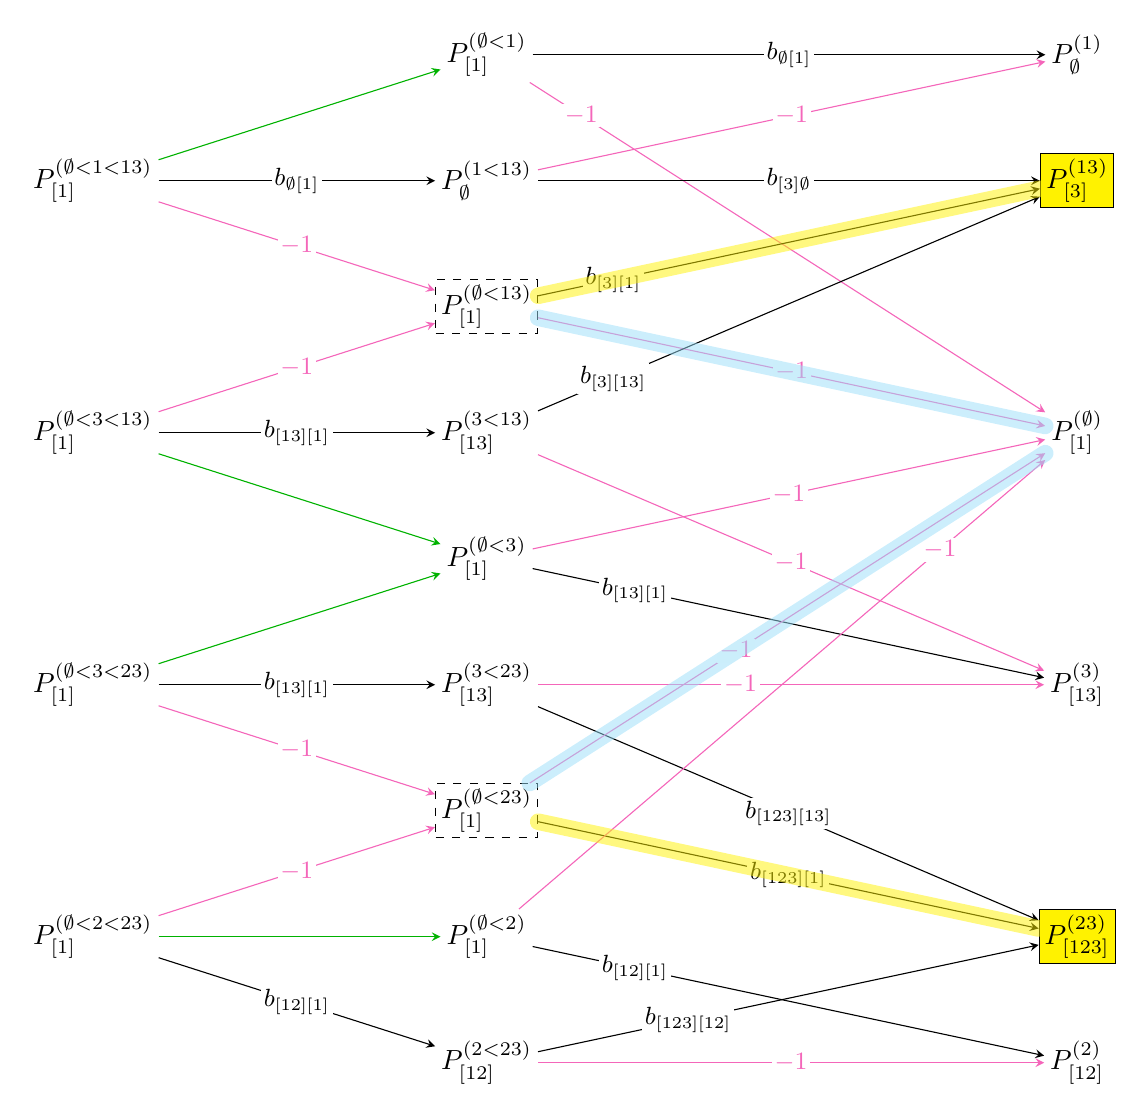
\begin{tikzpicture}[
  >=stealth,
  every node/.style={inner sep=2pt},
  labl/.style={fill=white, inner sep=1pt, font=\small}
]
\colorlet{pinkc}{magenta!60!white}
\colorlet{greenc}{green!70!black}

% Nodes (x = col*2.5cm, y = -row*1.6cm)
\node (P1-0-1-13)      at (2.5,-3.2)  {$P_{[1]}^{(\emptyset<1<13)}$};
\node (P1-0-3-13)      at (2.5,-6.4)  {$P_{[1]}^{(\emptyset<3<13)}$};
\node (P1-0-3-23)      at (2.5,-9.6)  {$P_{[1]}^{(\emptyset<3<23)}$};
\node (P1-0-2-23)      at (2.5,-12.8) {$P_{[1]}^{(\emptyset<2<23)}$};

\node (P1-0-1)        at (7.5,-1.6)  {$P_{[1]}^{(\emptyset<1)}$};
\node (P0-1-13)        at (7.5,-3.2)  {$P_{\emptyset}^{(1<13)}$};
\node[draw,dashed] (P1-0-13)        at (7.5,-4.8)  {$P_{[1]}^{(\emptyset<13)}$};
\node (P13-3-13)       at (7.5,-6.4)  {$P_{[13]}^{(3<13)}$};
\node (P1-0-3)         at (7.5,-8.0)  {$P_{[1]}^{(\emptyset<3)}$};
\node (P13-3-23)       at (7.5,-9.6)  {$P_{[13]}^{(3<23)}$};
\node[draw,dashed] (P1-0-23)        at (7.5,-11.2) {$P_{[1]}^{(\emptyset<23)}$};
\node (P1-0-2)         at (7.5,-12.8) {$P_{[1]}^{(\emptyset<2)}$};
\node (P12-2-23)       at (7.5,-14.4) {$P_{[12]}^{(2<23)}$};

\node (P0-1)           at (15,-1.6)   {$P_{\emptyset}^{(1)}$};
\node[draw,fill=yellow] (P3-13)          at (15,-3.2)   {$P_{[3]}^{(13)}$};
\node (P1-0)           at (15,-6.4)   {$P_{[1]}^{(\emptyset)}$};
\node (P13-3)          at (15,-9.6)   {$P_{[13]}^{(3)}$};
\node[draw,fill=yellow] (P123-23)        at (15,-12.8)  {$P_{[123]}^{(23)}$};
\node (P12-2)          at (15,-14.4)  {$P_{[12]}^{(2)}$};

% Arrows
\draw[->] (P1-0-1) -- node[labl]{$b_{\emptyset[1]}$} (P0-1);
\draw[->, color=pinkc] (P1-0-1) -- node[labl, pos=0.1]{$-1$} (P1-0);
\draw[->, color=greenc] (P1-0-1-13) -- (P1-0-1);
\draw[->] (P1-0-1-13) -- node[labl]{$b_{\emptyset[1]}$} (P0-1-13);
\draw[->, color=pinkc] (P1-0-1-13) -- node[labl]{$-1$} (P1-0-13);
\draw[->, color=pinkc] (P0-1-13) -- node[labl]{$-1$} (P0-1);
\draw[->] (P0-1-13) -- node[labl]{$b_{[3]\emptyset}$} (P3-13);
\draw[->] (P1-0-13) -- node[labl, pos=0.15]{$b_{[3][1]}$} (P3-13);
\draw[->, color=pinkc] (P1-0-13) -- node[labl]{$-1$} (P1-0);
\draw[->, color=pinkc] (P1-0-3-13) -- node[labl]{$-1$} (P1-0-13);
\draw[->] (P1-0-3-13) -- node[labl]{$b_{[13][1]}$} (P13-3-13);
\draw[->, color=greenc] (P1-0-3-13) -- (P1-0-3);
\draw[->] (P13-3-13) -- node[labl,pos=0.15]{$b_{[3][13]}$} (P3-13);
\draw[->, color=pinkc] (P13-3-13) -- node[labl]{$-1$} (P13-3);
\draw[->, color=pinkc] (P1-0-3) -- node[labl]{$-1$} (P1-0);
\draw[->] (P1-0-3) -- node[labl, pos=0.2]{$b_{[13][1]}$} (P13-3);
\draw[->, color=greenc] (P1-0-3-23) -- (P1-0-3);
\draw[->] (P1-0-3-23) -- node[labl]{$b_{[13][1]}$} (P13-3-23);
\draw[->, color=pinkc] (P1-0-3-23) -- node[labl]{$-1$} (P1-0-23);
\draw[->, color=pinkc] (P13-3-23) -- node[labl,pos=0.4]{$-1$} (P13-3);
\draw[->] (P13-3-23) -- node[labl]{$b_{[123][13]}$} (P123-23);
\draw[->, color=pinkc] (P1-0-23) -- node[labl,pos=0.4]{$-1$} (P1-0);
\draw[->] (P1-0-23) -- node[labl]{$b_{[123][1]}$} (P123-23);
\draw[->, color=pinkc] (P1-0-2-23) -- node[labl]{$-1$} (P1-0-23);
\draw[->, color=greenc] (P1-0-2-23) -- (P1-0-2);
\draw[->] (P1-0-2-23) -- node[labl]{$b_{[12][1]}$} (P12-2-23);
\draw[->, color=pinkc] (P1-0-2) -- node[labl, pos=0.8]{$-1$} (P1-0);
\draw[->] (P1-0-2) -- node[labl, pos=0.2]{$b_{[12][1]}$} (P12-2);
\draw[->] (P12-2-23) -- node[labl, pos=0.3]{$b_{[123][12]}$} (P123-23);
\draw[->, color=pinkc] (P12-2-23) -- node[labl]{$-1$} (P12-2);

\draw[line width=6pt, color=yellow, opacity=0.5, line cap=round, line join=round] (P1-0-13) -- (P3-13);
\draw[line width=6pt, color=yellow, opacity=0.5, line cap=round, line join=round] (P1-0-23) -- (P123-23);
\draw[line width=6pt, color=cyan!40!white, opacity=0.5, line cap=round, line join=round] (P1-0-13) -- (P1-0) -- (P1-0-23);
\end{tikzpicture}
    \caption{The complex $\mathcal{P}_\bullet$ for $I_{[1]}$ in the case when $\mathcal{J}(\{1<2\}\sqcup\{3\})$}
    \label{fig:complex-picture}
\end{figure}
\end{eg}

\medskip 

For each $Y\in\mathcal J(P)$, we have a free $R$-module $I_Xe_Y=D(e_YAe_X)$ of rank $1$.  Let $\phi_Y\colon P_Y\to I_X$ be the homomorphism determined by sending $e_Y$ to the canonical $R$-basis element dual to $b_{YX}\in e_YAe_X$. If $D_{Z_0}<D_{Z_1}$, then the corresponding distances are additive and $b_{Z_1Z_0}b_{Z_0X}=b_{Z_1X}$.  Consequently, $\phi_{Z_1}\mu_{Z_1,Z_0}=\phi_{Z_0}$ whenever $D_{Z_0}<D_{Z_1}$. Define
\[
 d_0:=\bigl(\phi_Y\bigr)_{Y\in\mathcal J(P)}\colon\mathcal P_0=\bigoplus_{Y\in\mathcal J(P)}P_Y\longrightarrow I_X.
\]
For \(D_{Z_0}<D_{Z_1}\), one has $d_0d_1\bigl(p^{(D_{Z_0}<D_{Z_1})}\bigr)=\phi_{Z_1}(b_{Z_1Z_0}p)-\phi_{Z_0}(p)=0$. Hence, by Proposition \ref{prop:resolution-differential}, we obtain a chain complex
\begin{equation}
 \widetilde{\mathcal{P}}_\bullet: \quad \cdots\longrightarrow\mathcal P_2\xrightarrow{d_2}\mathcal P_1\xrightarrow{d_1}\mathcal P_0\xrightarrow{d_0}I_X\longrightarrow0.
 \label{eq:candidate-complex}
\end{equation}
We call $\widetilde{\mathcal P}_\bullet$ the \defn{augmented candidate complex} and $\mathcal{P}_\bullet$ is its resolution part.

The main theorem we want to show is the following.
\begin{thm}\label{thm:exactness}
The complex $\widetilde{\mathcal{P}}_\bullet$ is exact, i.e. $\mathcal{P}_\bullet$ defines a projective resolution of $I_X$.
\end{thm}


Note that the projective resolution constructed above gives an upper bound on $\pdim_A I_X$ through the lengths of strict chains
in $\D_X$. Together with Corollary~\ref{cor:distance-gorenstein-criterion}, this yields the Iwanaga--Gorenstein property of $A$.

\begin{cor}\label{cor:distributive-ig}
For every $X\in\mathcal J(P)$, one has
\[
 \pdim_A I_X
 \leq\max\{d(X,Y)\mid D_Y\in\max\D_X\}
 \leq |P|.
\]
If $R$ is Gorenstein, then $A$ is a Gorenstein $R$-algebra. If $R$ is Iwanaga--Gorenstein, then $A$ is Iwanaga--Gorenstein and
\[
 \idim A_A=\idim {}_A A\leq |P|+\idim_R R.
\]
\end{cor}

\begin{proof}
Each summand of $\mathcal P_k$ is indexed by a strict chain $D_{Z_0}<\cdots<D_{Z_k}$, which extends to a maximal element $D_Y$ of $\D_X$. Thus $k\leq |D_Y|-|D_{Z_0}|\leq d(X,Y)\leq |P|$, and Theorem~\ref{thm:exactness} gives the projective dimension bound. The Gorenstein and Iwanaga--Gorenstein assertions follow from Corollary~\ref{cor:distance-gorenstein-criterion}.
\end{proof}

\bhx{(I think this fits better in the first paper, since orders have not been introduced here. I have placed it in Section~7.4 of that paper.)}

\bhx{
\comment{not sure if I want this in paper 1 instead...}
For every finite connected graph $G$, the distance algebra $\Sigma_G$ over a field $\Bbbk$ is isomorphic to $\Lambda_G/x\Lambda_G$ for an associated tiled $\Bbbk[[x]]$-order $\Lambda_G$; see \cite[Section~2.3]{CX26}. Combining Corollary~\ref{cor:distributive-ig} with \cite[Proposition~2.7]{CX26} gives the following family of Iwanaga--Gorenstein orders.

\begin{cor}\label{cor:tiled-orders-ig}
Let $\Bbbk$ be a field and let $L$ be a finite distributive lattice, with distance $\Bbbk$-algebra $\Sigma_L$. Then the associated tiled $\Bbbk[[x]]$-order $\Lambda_L$ is Iwanaga--Gorenstein, and
\[
 \idim (\Lambda_L)_{\Lambda_L}
 =\idim {}_{\Lambda_L}\Lambda_L
 =\idim (\Sigma_L)_{\Sigma_L}+1
 \leq\diam(L)+1.
\]
\end{cor}}

\subsection{Exactness of the candidate complex}
We prove exactness after right multiplication by each vertex idempotent $e_W$.  The first lemma records the multiplication criterion used in both steps of the argument.

\begin{lem}\label{lem:multiplication-criterion}
Let $W,Z,Y\in\mathcal J(P)$ with $D_Z\leq D_Y$.  Then
\[
 b_{YZ}b_{ZW}\neq0
 \quad\Longleftrightarrow\quad
 (D_Y\setminus D_Z)\cap D_W=\emptyset.
\]
\end{lem}

\begin{proof}
Since $b_{YZ}b_{ZW}\neq 0$ is equivalent to $d(W,Z)+d(Z,Y)=d(W,Y)$, it follows from Lemma~\ref{lem:d(X,Y)} that it is also equivalent to $D_W\SDiff D_Z = W\SDiff Z \subseteq  W\SDiff Y = D_W\SDiff D_Y$.  Since $D_Z\le D_Y$, we have $D_Z\setminus D_W \le D_Y\setminus D_W$, which means that
\begin{align*}
D_W\SDiff D_Z\subseteq D_W\SDiff D_Y  
\;\;\Leftrightarrow\;\; D_W\setminus D_Z \subseteq D_W\setminus D_Y 
\;\;\Leftrightarrow\;\; D_W \cap (D_Y\setminus D_Z) = \emptyset,
\end{align*}
as required.
\end{proof}

Fix $W\in\mathcal J(P)$.  Right multiplication by $e_W$ gives the complex
\begin{equation*}
 \widetilde{\mathcal P}_\bullet e_W:\quad
 \cdots\longrightarrow\mathcal P_1e_W
 \longrightarrow\mathcal P_0e_W
 \longrightarrow I_Xe_W\longrightarrow0.
\end{equation*}
We first replace it by a smaller homotopy equivalent subcomplex.

\begin{prop}\label{prop:lower-deformation-retract}
For $k\geq0$, put
\[
 \mathcal P_k^{\leq W}
 :=\bigoplus_{\substack{
 \sigma_\ast=(D_{Z_0}<\cdots<D_{Z_k})\in\Delta(\D_X)_k\\
 D_{Z_k}\leq D_W}}
 (P_{Z_0}e_W)^{(\sigma_\ast)}.
\]
Together with $I_Xe_W$ in degree $-1$, these $R$-modules form a subcomplex $\widetilde{\mathcal P}_\bullet^{\leq W}$ of $\widetilde{\mathcal P}_\bullet e_W$.  Its inclusion
\[
 \iota_W\colon
 \widetilde{\mathcal P}_\bullet^{\leq W}
 \longrightarrow
 \widetilde{\mathcal P}_\bullet e_W
\]
is a homotopy equivalence.
\end{prop}

\begin{proof}
Since $P_{Z_0}e_W=R\, b_{Z_0W}$, the differential in \eqref{eq:candidate-differential} evaluates to
\begin{equation}
 \begin{aligned}
 d_k\bigl((b_{Z_0W})^{(\sigma_\ast)}\bigr)
 &=\bigl(b_{Z_1Z_0}b_{Z_0W}\bigr)^{(\sigma_\ast^{\widehat0})}
 +\sum_{i=1}^k(-1)^i
 (b_{Z_0W})^{(\sigma_\ast^{\widehat i})}.
 \end{aligned}
 \label{eq:evaluated-differential}
\end{equation}
Deleting a member of a chain whose largest member is at most $D_W$ preserves this property, so the displayed $R$-modules form a subcomplex.

For $D_Z\in\D_X$, set $r_W(D_Z):=D_Z\cap D_W$. This again lies in $\D_X$: indeed, $M(Z,W):=(X\cap Z)\cup(X\cap W)\cup(Z\cap W)$ is an order ideal and satisfies $D_{M(Z,W)}=D_Z\cap D_W$.  Thus $r_W$ is an order-preserving map from $\D_X$ to $\D_{X,\leq W}$.

Fix $\sigma_\ast=(D_{Z_0}<\cdots<D_{Z_k})$ and let $T_i:=M(Z_i,W)$, so that $D_{T_i}=D_{Z_i}\cap D_W$.  Define $\rho_{W,-1}:=\id_{I_Xe_W}$ and, for $k\geq0$, define
\[
 \rho_{W,k}\bigl((b_{Z_0W})^{(\sigma_\ast)}\bigr)
 :=
 \begin{cases}
 (b_{T_0W})^{(D_{T_0}<\cdots<D_{T_k})},
     &D_{T_0}<\cdots<D_{T_k},\\
 0,&D_{T_i}=D_{T_{i+1}}\text{ for some }i.
 \end{cases}
\]
Then $\rho_W\iota_W=\id$ as graded maps.

It remains to construct the homotopy.  Put $h_{W,-1}:=0$ and, for $k\geq0$, define
\begin{equation*}
 \begin{aligned}
 h_{W,k}\bigl((b_{Z_0W})^{(\sigma_\ast)}\bigr)
 :=\sum_{j=0}^k(-1)^j
 (b_{T_0W})^{(
 D_{T_0}\leq\cdots\leq D_{T_j}\leq
 D_{Z_j}<\cdots<D_{Z_k})}.
 \end{aligned}
\end{equation*}
A summand is understood to be zero if two adjacent members of its indexing sequence are equal.  We now suppress the subscript $W$ from $\iota$, $\rho$, and $h$.

For $k=0$, a direct calculation gives $d_1h_0 =\id_{\mathcal P_0e_W}-\iota_0\rho_0$. For $k\geq1$, put
\[
 \tau_j
 :=(D_{T_0}\leq\cdots\leq D_{T_j}\leq
 D_{Z_j}<\cdots<D_{Z_k}).
\]
Expanding the differential gives
\[
 \begin{aligned}
 d_{k+1}h_k\bigl((b_{Z_0W})^{(\sigma_\ast)}\bigr)
 &=(b_{Z_0T_0}b_{T_0W})^{(\sigma_\ast)}\\
 &\quad+\sum_{j=1}^k(-1)^j
 (b_{T_1T_0}b_{T_0W})^{(\tau_j^{\widehat0})}\\
 &\quad+\sum_{j=0}^k\sum_{i=1}^{k+1}(-1)^{i+j}
 (b_{T_0W})^{(\tau_j^{\widehat i})}.
 \end{aligned}
\]
Because $(D_U\setminus r_W(D_U))\cap D_W=\emptyset$, Lemma~\ref{lem:multiplication-criterion} gives $b_{Z_iT_i}b_{T_iW}=b_{Z_iW}$.  The first term is therefore the original basis element, the single sum is $-h_{k-1}\bigl( (b_{Z_1Z_0}b_{Z_0W})^{(\sigma_\ast^{\widehat0})} \bigr)$, and the double sum is
\[
 -\sum_{\ell=1}^k(-1)^\ell
 h_{k-1}\bigl((b_{Z_0W})^{(\sigma_\ast^{\widehat\ell})}\bigr)
 -\iota_k\rho_k\bigl((b_{Z_0W})^{(\sigma_\ast)}\bigr).
\]
Comparing this with the expansion of $h_{k-1}d_k$ yields
\begin{equation*}
 d_{k+1}h_k+h_{k-1}d_k
 =\id_{\mathcal P_ke_W}-\iota_k\rho_k
 \qquad(k\geq0).
\end{equation*}
For $k\geq1$, applying $d_k$ to this identity and comparing with the identity in degree $k-1$ gives
\[
 d_k(\id-\iota_k\rho_k)
 =(\id-\iota_{k-1}\rho_{k-1})d_k.
\]
Since $\iota_W$ is an injective chain map, it follows that $d_k\rho_k=\rho_{k-1}d_k$.  The same conclusion in degree zero follows by applying $d_0$ to the degree-zero homotopy identity.  Thus $\rho_W$ is a chain map and the displayed identity is the required homotopy.
\end{proof}

The lower subcomplex admits a direct decomposition into augmented chain complexes of intervals.

\begin{prop}\label{prop:lower-subcomplex-exact}
For every $W\in\mathcal J(P)$, the complex $\widetilde{\mathcal P}_\bullet^{\leq W}$ is exact.
\end{prop}

\begin{proof}
For $D_Y\leq D_W$ and $k\geq0$, put
\[
 K_{Y,k}
 :=\bigoplus_{\substack{
 \sigma_\ast=(D_Y<D_{Z_1}<\cdots<D_{Z_k})\in\Delta(\D_X)_k\\
 D_{Z_k}\leq D_W}}
 (P_Ye_W)^{(\sigma_\ast)}.
\]
If $D_Y<D_{Z_1}\leq D_W$, then $(D_{Z_1}\setminus D_Y)\cap D_W\neq\emptyset$.  Hence Lemma~\ref{lem:multiplication-criterion} gives $b_{Z_1Y}b_{YW}=0$, and \eqref{eq:evaluated-differential} shows that $K_{Y,\bullet}$ is a subcomplex.

If $D_Y<D_W$, then the restriction of $d_0$ to $K_{Y,0}$ is zero by Lemma~\ref{lem:d(X,Y)}.
%Indeed, by Lemma \ref{lem:d(X,Y)} we have
%\[
% \left.\phi_Y\right|_{P_Ye_W}\neq0
% \quad\Longleftrightarrow\quad
% d(X,Y)=d(X,W)+d(W,Y)
% \quad\Longleftrightarrow\quad
% D_W\leq D_Y,
%\]
%which is impossible when $D_Y<D_W$.
Now let $\D_{X,Y,W}:=\{D_T\in\D_X\mid D_Y<D_T\leq D_W\}$. Deleting the initial member of an indexing chain in each $K_{Y,k}$ for $k>0$ and sending $b_{YW}^{(D_Y)} \in K_{Y,0}$ to $1\in C_{-1}(\Delta(\D_{X,Y,W}))$ defines an isomorphism of chain complexes
\[
 K_{Y,\bullet}
 \xrightarrow{\sim}
 \widetilde C_\bullet
 \bigl(\Delta(\D_{X,Y,W})\bigr)[1].
\]  
%It is straightforward to check that the signs agree with \eqref{eq:evaluated-differential}.  
Since $D_W$ is the maximum of $\D_{X,Y,W}$, its order complex is a cone and its augmented chain complex is exact.

When $D_Y=D_W$, one has $Y=W$.  The complex $K_{W,\bullet}$ is concentrated in degree zero, and $d_0=\phi_We_W\colon K_{W,0}\longrightarrow I_Xe_W$ is a homomorphism between free $R$-modules of rank one sending the canonical basis element to the canonical dual basis element, hence an isomorphism.  Therefore
\[
 \widetilde{\mathcal P}_\bullet^{\leq W}
 =\left(\bigoplus_{D_Y<D_W}K_{Y,\bullet}\right)
 \oplus\left(K_{W,0}\xrightarrow{\sim}I_Xe_W\right)
\]
is a direct sum of exact complexes.
\end{proof}

\begin{proof}[Proof of Theorem~\ref{thm:exactness}]
For every $W\in\mathcal J(P)$, Proposition~\ref{prop:lower-deformation-retract} identifies $\widetilde{\mathcal P}_\bullet e_W$, up to homotopy, with the exact complex $\widetilde{\mathcal P}_\bullet^{\leq W}$ from Proposition~\ref{prop:lower-subcomplex-exact}.  Hence every $\widetilde{\mathcal P}_\bullet e_W$ is exact, and so taking the direct sum over $W\in \mathcal{J}(P)$ yields an exact complex $\widetilde{\mathcal P}_\bullet =\bigoplus_{W\in\mathcal J(P)} \widetilde{\mathcal P}_\bullet e_W$.
\end{proof}

\begin{eg}\label{subsec:eg3}
We continue with Examples~\ref{subsec:eg1} and~\ref{subsec:eg2}. Put $W=[13]$, so $D_W=\{3\}$.  Right multiplication by $e_W$ gives

\[
 \mathcal P_\bullet e_W:
 0\longrightarrow\mathcal P_2e_W\xrightarrow{d_2e_W}\mathcal P_1e_W\xrightarrow{d_1e_W}\mathcal P_0e_W\xrightarrow{d_0e_W}I_{[1]}e_W\longrightarrow0.
\]

Explicitly, $\mathcal P_ke_W$ is obtained from the displayed expression for $\mathcal P_k$ by replacing every labelled copy $P_Z^{(\sigma_\ast)}$ by $P_Ze_W^{(\sigma_\ast)}$.  The lower subcomplex consists of the labelled copies for which every member of $\sigma_\ast$ is contained in $D_W=\{3\}$.  It is
\[
 0\longrightarrow(P_{[1]}e_{[13]})^{(\emptyset<\{3\})}\xrightarrow{d_1}(P_{[1]}e_{[13]})^{(\emptyset)}\oplus(P_{[13]}e_{[13]})^{(\{3\})}\xrightarrow{d_0}I_{[1]}e_{[13]}\longrightarrow0.
\]
For $p\in P_{[1]}e_{[13]}$, its first differential is
\[
 d_1\bigl(p^{(\emptyset<\{3\})}\bigr)=\bigl(b_{[13],[1]}p\bigr)^{(\{3\})}-p^{(\emptyset)}.
\]
In particular, for the path class $b_{[1],[13]}\in P_{[1]}e_{[13]}$,
\[
 d_1\bigl((b_{[1],[13]})^{(\emptyset<\{3\})}\bigr)=-(b_{[1],[13]})^{(\emptyset)},
\]
because $b_{[13],[1]}b_{[1],[13]}=0$. In the indicated bases, the augmented lower subcomplex is
\[
 0\longrightarrow R\xrightarrow{\binom{-1}{0}}R^2\xrightarrow{(0\;1)}R\longrightarrow0.
\]
\end{eg}


%%%%%%%%%%%%%%%%%%%%%%%%%%%%%%%%%%%%%%%%%%%%%%%%%%%%%%%%%%%%%
%%%%%%%%%%%%%%%%%%%%%%%%%%%%%%%%%%%%%%%%%%%%%%%%%%%%%%%%%%%%%

\section{Morse reduction and the minimal projective resolution}
\label{sec:minimal-morse}

While we now know that ${\mathcal P}_\bullet$ is a projective resolution of $I_X$, it is far from being minimal.  To obtain a minimal resolution, we apply algebraic Morse theory \cite{CLZ26} to remove its invertible differential components.  
Throughout, we require the ground ring $R=\Bbbk$ to be a field.

\subsection{Algebraic Morse theory}
\label{subsec:algebraic-morse}

Roughly speaking, for a complex $(X_\bullet, d)$ that comes with a special gadget $\mathcal{M}$ called Morse matching, algebraic Morse theory says that we can obtain a `smaller' complex $(X_\bullet^{\mathcal M}, d^{\mathcal M})$ that is homotopic to $(X,d)$ by identifying terms appearing in a Morse matching appropriately.
This usage of algebraic Morse theory we use follows \cite[Section~3]{CLZ26}.

\begin{dfn}\label{dfn:morse-matching}
Let $(X_\bullet,d)$ be a complex of right $A$-modules with fixed decompositions $X_n=\bigoplus_{\alpha\in I_n}X_{n,\alpha}$.
Write $d_{\beta,\alpha}\colon X_{n,\alpha}\to X_{n-1,\beta}$ for the matrix components of $d_n$.
\begin{enumerate}
\item The \defn{weighted quiver} $Q(X_\bullet)$ has the summands $X_{n,\alpha}$ as vertices and an arrow $X_{n,\alpha}\xrightarrow{d_{\beta,\alpha}}X_{n-1,\beta}$ weighted by $d_{\beta,\alpha}$ whenever $d_{\beta,\alpha}\neq0$.

\item A \defn{partial matching} $\mathcal M$ is a collection of arrows such that
\begin{enumerate}
\item no two selected arrows share a vertex;
\item the weight of every selected arrow is an isomorphism.
\end{enumerate}

\item Form a new weighted quiver $Q^{\mathcal M}$ by
%\begin{enumerate}
%\item \bhx{retaining every unmatched arrow and drawing it as a \defn{thick} arrow;} \comment{I question what is the point of this terminology... just `unmatched' arrow is fine???}
%\item
replacing each matched arrow $W\xrightarrow{w}U$ by a \defn{dotted} arrow $U\to W$ in reverse direction of weight $-w^{-1}$.
%\end{enumerate}
A vertex not incident with a matched arrow is called \defn{critical}.

\item A directed path in $Q^{\mathcal M}$ is a \defn{zigzag path} if thick and dotted arrows alternate; a path consisting of one arrow is also allowed.  We shall use the following single path notation.  For a vertex $U$ in degree $n$ and a vertex $V$ in degree $n-1$, let $\Gamma_n^{\mathcal M}(U,V)$ be the set of zigzag paths from $U$ to $V$ of the form
\[
 U=U_0\morsethickarrow U_1
 \morsedottedarrow U_2
 \morsethickarrow\cdots
 \morsedottedarrow U_{2r}
 \morsethickarrow U_{2r+1}=V,
 \qquad r\geq0.
\]
The weight $\weight(\gamma)$ of a zigzag path $\gamma$ is the composition, along the order of the zigzag path $\gamma$, of the weights of its arrows.

\item The partial matching $\mathcal M$ is a \defn{Morse matching} if it satisfies the following local finiteness hypothesis: for every matched arrow $W\xrightarrow{w}U$, every vertex $V$ in the same degree, say, $n-1$ as $U$, and every $x\in U$, the sum
\[
 \sum_{\gamma\in\Gamma_n^{\mathcal M}(W,V)}
 \weight(\gamma)\bigl(-w^{-1}(x)\bigr)
\]
is well-defined, and it is non-zero for only finitely many vertices $V$.
\end{enumerate}
\end{dfn}

One special case where the the local finiteness hypothesis  can be conveniently verified is the following.

\begin{prop}\textnormal{(\cite[Proposition~3.2]{CLZ26})}
\label{prop:morse-sufficient-condition}
Let $\mathcal M$ be a partial matching of $Q(X_\bullet)$.  If $Q^{\mathcal M}$ contains no infinite zigzag path, then $\mathcal M$ is a Morse matching.
\end{prop}

We next record the main result of algebraic Morse theory.

\begin{thm}\textnormal{(\cite[Theorem~3.3]{CLZ26})}
\label{thm:algebraic-morse}
Let $\mathcal M$ be a Morse matching of $Q(X_\bullet)$, and write $\Crit_n(\mathcal M)$ for its critical vertices in degree $n$.  Then we have complex $(X_\bullet^{\mathcal{M}},d^{\mathcal{M}})$, called \defn{Morse complex}, given by
\[
 X_n^{\mathcal M}
 :=\bigoplus_{U\in\Crit_n(\mathcal M)}U,  \qquad d_{V,U}^{\mathcal M}
 :=\sum_{\gamma\in\Gamma_n^{\mathcal M}(U,V)} \weight(\gamma),
\]
where $d^{\mathcal{M}}_{V,U}$ is the $(V,U)$-component of $d_n^{\mathcal{M}}:X_n^{\mathcal{M}}\to X_{n-1}^{\mathcal{M}}$ for $U\in\Crit_n(\mathcal M)$ and $V\in\Crit_{n-1}(\mathcal M)$.
%For critical vertices $U$ in degree $n$ and $V$ in degree $n-1$, define the $(V,U)$-component of $d_n^{\mathcal M}\colon X_n^{\mathcal M}\to X_{n-1}^{\mathcal M}$ by
%\[
% d_{V,U}^{\mathcal M}
% :=\sum_{\gamma\in\Gamma^{\mathcal M}(U,V)}
% \weight(\gamma).
%\]
%Then $(X_\bullet^{\mathcal M},d^{\mathcal M})$ is a complex.  
Moreover, it is homotopy equivalent to $(X_\bullet,d)$ -- more precisely, one has a decomposition of chain complexes
\[
 (X_\bullet,d)\cong
 (X_\bullet^{\mathcal M},d^{\mathcal M})
 \oplus(Y_\bullet,d^Y),
\]
where $Y_\bullet$ is null-homotopic.
\end{thm}

In particular, if $X_\bullet$ is a projective resolution of a module, then its Morse complex is also a projective resolution of the same module.

\subsection{Construction of the Morse matching}
\label{subsec:construction-morse-matching}

Let us first explain the idea of how to find a Morse matching.
The differential formula~\eqref{eq:candidate-differential} separates the faces of a strict chain into two types: the zeroth face deletes its initial member, whereas the remaining faces preserve the initial member.  Under the identification~\eqref{eq:candidate-terms}, these two contributions give a decomposition $d=\delta+\partial$, where the non-zero components of $\partial$ are signed identity maps between copies of the same projective, while those of $\delta$ is induced by the left-multiplication map (more precise formulation will come after the next paragraph).

The difficulty of finding a Morse matching is that the signed identity components of $\partial$ need not themselves form a partial matching, since several of them may share a source or target (see Example \ref{subsec:eg2}).
The `solution' is to do what usual homological perturbation theory does: decompose using a choice of kernel--image splitting for each chain complex $C_\bullet(\Delta_Z)$.  
With respect to this new choice of decomposition, the matrix components of both $\partial$ and $\delta$ will change, but $\partial$ becomes a collection of isomorphisms with pairwise disjoint endpoints, whereas every matrix component arising from $\delta$ are still radical maps.  The former components will define the Morse matching, and the latter property will control its zigzag paths.

\medskip

\bhx{We now construct the matching.} All tensor products below are over $\Bbbk$. For $Z\in\mathcal J(P)$, put
\[
 C_{Z,\bullet}:=\widetilde C_\bullet(\Delta_Z)[1],
 \qquad C_{Z,k}=\widetilde C_{k-1}(\Delta_Z),
 \qquad \partial^Z_k:C_{Z,k}\longrightarrow C_{Z,k-1},
\]
where $\partial^Z_k$ is the negative of the reduced simplicial
boundary. Thus $C_{Z,0}=\Bbbk 1_Z$, $C_{Z,k}=0$ for $k<0$,
and $\partial^Z_0=0$.

For $D_Z<D_T$ and $k\geq1$, define
$\delta_{T,Z,k}:C_{Z,k}\to C_{T,k-1}$ on the standard basis by
\[
 \delta_{T,Z,k}\langle D_{Z_1}<\cdots<D_{Z_k}\rangle
 =
 \begin{cases}
  1_T,&T=Z_1\text{ and }k=1,\\
  \langle D_{Z_2}<\cdots<D_{Z_k}\rangle,
       &T=Z_1\text{ and }k>1,\\
  0,&T\neq Z_1.
 \end{cases}
\]
Here $D_Z<D_{Z_1}<\cdots<D_{Z_k}$; when $T=Z_1$, the output
is a basis element of $C_{T,k-1}$. Under
\eqref{eq:candidate-terms}, we have, for $k\geq1$,
\[
 \begin{aligned}
 d_k&=\partial_k+\delta_k:
       \mathcal P_k\longrightarrow\mathcal P_{k-1},\\
 \partial_k&:=\bigoplus_Z\id_{P_Z}\otimes\partial^Z_k,
 \qquad
 \delta_k:=\sum_{D_Z<D_T}\mu_{T,Z}\otimes\delta_{T,Z,k}.
 \end{aligned}
\]
The $(T,Z)$-component of $\delta_k$ has source
$P_Z\otimes C_{Z,k}$ and target $P_T\otimes C_{T,k-1}$.
Recall that $\mu_{T,Z}:P_Z\to P_T$ is given by $p\mapsto b_{TZ}p$.

More explicitly, a full chain
$\sigma_\ast=(D_Z<D_{Z_1}<\cdots<D_{Z_k})$ labels a copy of
$P_Z$, namely,
$P_Z\otimes\Bbbk\langle\sigma_\ast^{\widehat0}\rangle$.
The map $\partial_k$ deletes $D_{Z_i}$ from $\sigma_\ast$
for $1\leq i\leq k$, with coefficient $(-1)^i$;
its image remains in $P_Z\otimes C_{Z,k-1}$.
The map $\delta_k$ deletes $D_Z$ from $\sigma_\ast$.
The resulting full chain starts at $D_{Z_1}$, so its tensor
representation belongs to $P_{Z_1}\otimes C_{Z_1,k-1}$
and has tail $\langle D_{Z_2}<\cdots<D_{Z_k}\rangle$.
For $k=1$, the tail is meant to be $1_{Z_1}$.

Since $\Bbbk$ is a field, choose, for every $Z$ and $k\geq0$,
a decomposition
\begin{equation}
 \begin{gathered}
 C_{Z,k}=B_{Z,k}\oplus H_{Z,k}\oplus L_{Z,k},\qquad 
\text{ where } B_{Z,k}:=\Image\partial^Z_{k+1},\text{ and }
 B_{Z,k}\oplus H_{Z,k}=\Ker\partial^Z_k,\\
 \left.\partial^Z_k\right|_{L_{Z,k}}:
 L_{Z,k}\xrightarrow{\sim}B_{Z,k-1}\qquad(k\geq1).
 \end{gathered}
 \label{eq:homology-splitting}
\end{equation}
In particular, $L_{Z,0}=0$, and the canonical projection from $\Ker \partial_k^Z$
restricts to an isomorphism
\[
 H_{Z,k}\xrightarrow{\sim}H_k(C_{Z,\bullet})
 \cong\widetilde H_{k-1}(\Delta_Z),\qquad h\longmapsto h+B_{Z,k}.
\]
Use the resulting decomposition
\[
 \mathcal P_k=\bigoplus_{Z\in\mathcal J(P)}
 \bigl((P_Z\otimes B_{Z,k})\oplus
       (P_Z\otimes H_{Z,k})\oplus
       (P_Z\otimes L_{Z,k})\bigr)
\]
to form the weighted quiver of the resolution part
$\mathcal P_\bullet$, that is, the vertices of the weighted quiver at degree $k$ are given by $(Z,E)$ for $Z\in\matcal{J}(P)$ and $E\in\{B,H,L\}$ such that the summand $P_Z\otimes E_{Z,k}$ is non-zero.  Note that the map $\partial_k$ sends $P_Z\otimes C_{Z,k}$ into $P_Z\otimes C_{Z,k-1}$, whereas $\delta_k$ sends it into $\bigoplus_{D_Z<D_T}P_T\otimes C_{T,k-1}$.

Define $\mathcal M$ by selecting all nonzero components
\begin{equation}
 \id_{P_Z}\otimes\left.\partial^Z_k\right|_{L_{Z,k}}:
 P_Z\otimes L_{Z,k}\xrightarrow{\sim}P_Z\otimes B_{Z,k-1}
 \qquad(k\geq1).
 \label{eq:morse-matching}
\end{equation}
These are precisely the nonzero components of $\partial$:
$\partial^Z_k$ vanishes on $B_{Z,k}\oplus H_{Z,k}$ and
maps $L_{Z,k}$ onto $B_{Z,k-1}$. Both the source $P_Z\otimes L_{Z,k}$ and the target $P_Z\otimes B_{Z,k-1}$ of each displayed map have label $Z$. Since every nonzero component of $\delta_k$ changes the label from $Z$ to some $T$ with $D_Z<D_T$, the component
of $\delta_k$ between these two summands is zero.
Hence the component of $d_k=\partial_k+\delta_k$ from
$P_Z\otimes L_{Z,k}$ to $P_Z\otimes B_{Z,k-1}$ is exactly
$\id_{P_Z}\otimes\left.\partial^Z_k\right|_{L_{Z,k}}$. Their endpoints are pairwise disjoint and their weights are isomorphisms, so $\mathcal M$ is a partial matching.

\begin{thm}\label{thm:minimal-resolution}
The partial matching $\mathcal M$ in \eqref{eq:morse-matching}
is a Morse matching. Its Morse complex defines a minimal
projective resolution
\[
 \cdots\longrightarrow\mathcal P_{\min,2}
 \longrightarrow\mathcal P_{\min,1}
 \longrightarrow\mathcal P_{\min,0}
 \longrightarrow I_X\longrightarrow0
\]
whose terms, for $k\geq0$, are
\begin{equation}
 \begin{aligned}
 \mathcal P_{\min,k}
 &=\bigoplus_{Z\in\mathcal J(P)}P_Z\otimes H_{Z,k} \cong\bigoplus_{Z\in\mathcal J(P)}
 P_Z\otimes\widetilde H_{k-1}(\Delta_Z)
 \cong\bigoplus_{Z\in\mathcal J(P)}
 P_Z^{\oplus\widetilde\beta_{Z,k}},
 \end{aligned}
 \label{eq:minimal-terms}
\end{equation}
where $\widetilde\beta_{Z,k}:=
\dim_{\Bbbk}\widetilde H_{k-1}(\Delta_Z)$.
\end{thm}
\comment{TODO: ask GPT if top degree $\mathcal{P}_k$ always vanish in minimal.  i.e $\beta_{Z,k}=0$ for all $Z$ when $k=|P|$?}

\begin{proof} 
\comment{refine language}
We first verify that $\mathcal{M}$ is a Morse matching.
Every dotted arrow in $Q^{\mathcal M}$ is of the form
\[
 P_Z\otimes B_{Z,k-1}\longrightarrow P_Z\otimes L_{Z,k},
 \qquad
 -\id_{P_Z}\otimes
 \left(\left.\partial^Z_k\right|_{L_{Z,k}}\right)^{-1}.
\]
Both endpoints belong to blocks labelled by the same $Z$.
Every thick arrow is a component of $\delta$, hence has the form
\[
 P_Z\otimes E_{Z,k}
 \xrightarrow{\mu_{T,Z}\otimes \delta'_{T,Z}}
 P_T\otimes F_{T,k-1},
 \qquad D_Z<D_T,
\]
where $E,F\in\{B,H,L\}$ and
$\delta'_{T,Z}:E_{Z,k}\to F_{T,k-1}$ is the composition
\begin{equation}\label{eq:delta'}
 \delta'_{T,Z}:E_{Z,k}\hookrightarrow C_{Z,k}
 \xrightarrow{\delta_{T,Z,k}}C_{T,k-1}
 \twoheadrightarrow F_{T,k-1}.
\end{equation}
Thus, along any zigzag path, dotted arrows preserve the
block label $D_Z$, while successive thick arrows determine
a strict chain $D_{Z_0}<D_{Z_1}<\cdots<D_{Z_r}$ in $\D_X$.
There are at most $|\D_X|-1$ thick arrows and at most $|\D_X|$ dotted arrows. In particular, there is no infinite zigzag path. Proposition~\ref{prop:morse-sufficient-condition}
therefore shows that $\mathcal M$ is a Morse matching.

Note that the critical summands in degree $k$ are precisely the
nonzero $P_Z\otimes H_{Z,k}$. By
Theorem~\ref{thm:algebraic-morse}, the Morse complex has
the terms in \eqref{eq:minimal-terms} and is homotopy
equivalent to $\mathcal P_\bullet$. Its terms are projective,
so Theorem~\ref{thm:exactness} shows that it defines a
projective resolution of $I_X$.

Now it remains to show that the Morse complex is minimal.
Put $J:=\rad A$. Fix $k\geq1$ and a zigzag path $\gamma$
from the critical summand $P_Z\otimes H_{Z,k}$ to the
critical summand $P_T\otimes H_{T,k-1}$.
The last arrow of $\gamma$ is thick, since no dotted arrow
is incident with a critical summand. It therefore has the form
\[
 P_U\otimes E_{U,k}
 \xrightarrow{\mu_{T,U}\otimes \delta'_{T,U}}
 P_T\otimes H_{T,k-1},
 \qquad D_U<D_T,
\]
where $U\in\mathcal J(P)$, $E\in\{B,H,L\}$, and
$\delta_{T,U}':E_{U,k}\to H_{T,k-1}$ is as defined in \eqref{eq:delta'}.
Since $U\neq T$, we have $b_{TU}\in J$, and
$\mu_{T,U}(p)=b_{TU}p\in e_TJ=P_TJ$ for every $p\in P_U$.
The last arrow therefore has image in
$(P_TJ)\otimes H_{T,k-1}$, and consequently
\[
 \Image\weight(\gamma)
 \subseteq(P_TJ)\otimes H_{T,k-1}
 =(P_T\otimes H_{T,k-1})J.
\]
By the path formula in Theorem~\ref{thm:algebraic-morse},
each component of $d_{\min,k}$ is a finite sum of such
weights. Summing over all target critical summands gives
\[
 \Image d_{\min,k}\subseteq\mathcal P_{\min,k-1}J
 \qquad(k\geq1).
\]
Thus, the differential $d_{\min}$ is radical at every degree, which shows the required minimality.
\end{proof}



This yields a refinement of Corollary \ref{cor:distributive-ig}.

\begin{cor}\label{cor:SigmaJ(P) is IG}
For the $\Bbbk$-algebra $\Sigma_L$ assocaited to a finite distributive lattice $L$, the projective dimension of the indecomposable injective $\Sigma_L$-module $I_X$ is
\begin{align}
 \pdim_{\Sigma_L} I_X
 &=\max\left\{k\geq0\ \middle|\
 \widetilde H_{k-1}(\Delta_Z)\neq0
 \text{ for some }Z\in\mathcal J(P)\right\}
 \label{eq:projective-dimension}\\
 &\leq\max\{d(X,Y)\mid D_Y\in\max\D_X\}.\notag
\end{align}
In particular, $\Sigma_L$ is Iwanaga--Gorenstein with self-injective dimension bounded above by $|P|$.
\end{cor}

\begin{proof}
Equation~\eqref{eq:projective-dimension} follows from the minimal terms in \eqref{eq:minimal-terms}. 
The rest are immediate from Corollary \ref{cor:distributive-ig} in the special case when $R=\Bbbk$.
\end{proof}

\begin{rmk}
The multiplicities in \eqref{eq:minimal-terms} can also be checked directly from Ext groups.  Fix $Z\in\mathcal J(P)$.  Since \eqref{eq:candidate-complex} is a projective resolution, $\Ext_A^k(I_X,S_Z)=H^k\Hom_A(\mathcal P_\bullet,S_Z)$.
For $T\in\mathcal J(P)$,
\[
 \Hom_A(P_T,S_Z)\cong
 \begin{cases}
  \Bbbk,&T=Z,\\
  0,&T\neq Z.
 \end{cases}
\]
Consequently, the degree-$k$ term of $\Hom_A(\mathcal P_\bullet,S_Z)$ has a basis indexed by the chains $D_Z<D_{Z_1}<\cdots<D_{Z_k}$.
The component of $d_k$ deleting $D_Z$ has target $P_{Z_1}$ and vanishes after applying $\Hom_A(-,S_Z)$.  The remaining components are the signed identity maps.  Hence this cochain complex is, up to a degree shift and signs, dual to \eqref{eq:reduced-chain-complex} for $\Delta_Z$.  Therefore
\[
 \dim_{\Bbbk}\Ext_A^k(I_X,S_Z)
 =\dim_{\Bbbk}\widetilde H_{k-1}(\Delta_Z),
\]
in agreement with the critical summands of the Morse matching.
\end{rmk}

The choices in \eqref{eq:homology-splitting} may change the individual differentials in the Morse complex.  Nevertheless, the resulting complexes are minimal projective resolutions of the same module and are therefore isomorphic.  In particular, $P_Z$ occurs in degree $k$ precisely when $\widetilde H_{k-1}(\Delta_Z)\neq0$.



\begin{eg}\label{eg:morse-matching-change-of-basis}
Continue with Examples~\ref{subsec:eg1} and~\ref{subsec:eg2}.  
We can regard Figure~\ref{fig:complex-picture} as the weighte quiver with respect to the standard decomposition of $\mathcal{P}_k$ indexed by chains in $\Delta(\D_X)$.  
Let us demonstrate the alternative choice used in Theorem \ref{thm:minimal-resolution}.

For $Z=[1]$, take
\begin{align*}
 L_{[1],2}=C_{[1],2}
  =\Bbbk\{&
  \langle\underline{1}<\underline{13}\rangle,
  \langle\underline{3}<\underline{13}\rangle,
  \langle\underline{3}<\underline{23}\rangle,
  \langle\underline{2}<\underline{23}\rangle\},\\
 B_{[1],1}=\Bbbk\{&
  \langle\underline{1}\rangle-\langle\underline{13}\rangle,
  \langle\underline{3}\rangle-\langle\underline{13}\rangle,
  \langle\underline{3}\rangle-\langle\underline{23}\rangle,
  \langle\underline{2}\rangle-\langle\underline{23}\rangle\},\\
 L_{[1],1}={}&\Bbbk\{\langle\underline{13}\rangle\}.
\end{align*}
For the remaining indices with non-zero degree one terms, take
\begin{align*}
 L_{\emptyset,1}&=\Bbbk\{\langle\underline{13}\rangle\},
 &L_{[12],1}&=\Bbbk\{\langle\underline{23}\rangle\},\\
 L_{[13],1}&=\Bbbk\{\langle\underline{13}\rangle\},
 &H_{[13],1}&=
 \Bbbk\{\langle\underline{13}\rangle-
              \langle\underline{23}\rangle\},\\
 B_{Z,0}&=C_{Z,0}
 &&(Z=[1],\emptyset,[12],[13]),\\
 H_{Z,0}&=C_{Z,0}
 &&(Z=[3],[123]).
\end{align*}
All unlisted spaces in the decomposition
\eqref{eq:homology-splitting} are zero.

The restriction of the internal differential to $L_{[1],2}$ is given by
\begin{align*}
 \langle\underline{1}<\underline{13}\rangle
   &\longmapsto
   \langle\underline{1}\rangle-\langle\underline{13}\rangle,&
 \langle\underline{3}<\underline{13}\rangle
   &\longmapsto
   \langle\underline{3}\rangle-\langle\underline{13}\rangle,\\
 \langle\underline{3}<\underline{23}\rangle
   &\longmapsto
   \langle\underline{3}\rangle-\langle\underline{23}\rangle,&
 \langle\underline{2}<\underline{23}\rangle
   &\longmapsto
   \langle\underline{2}\rangle-\langle\underline{23}\rangle.
\end{align*}
Moreover, $\partial^Z_1$ sends the displayed generator of each
$L_{Z,1}$ to $-1\in B_{Z,0}$.  These eight isomorphisms have pairwise
disjoint endpoints and are selected for the Morse matching.  This makes
explicit how the green arrows of Figure~\ref{fig:complex-picture} are
combined by the change of basis.

The matrix components of $\delta$ also change.  For example, $
 \delta_2\bigl(
 p\otimes\langle\underline{3}<\underline{23}\rangle
 \bigr)
 =b_{[13][1]}p\otimes\langle\underline{23}\rangle,
$ and, in the chosen decomposition of $C_{[13],1}$, we get that
$\langle\underline{23}\rangle
 =\langle\underline{13}\rangle
  -\bigl(
    \langle\underline{13}\rangle-
    \langle\underline{23}\rangle
   \bigr)$.
It thus produces two matrix components, of weights
$b_{[13][1]}$ and $-b_{[13][1]}$, respectively.  Similarly,
\[
 \delta_1\bigl(
 p\otimes(
 \langle\underline{3}\rangle-\langle\underline{13}\rangle)
 \bigr)
 =b_{[13][1]}p\otimes1-b_{[3][1]}p\otimes1.
\]
These are precisely the corresponding arrows displayed in Figure~\ref{fig:morse-matching-change-of-basis}, where we write $P_Z\langle c\rangle:=P_Z\otimes_{\Bbbk}\Bbbk c$ for compactness.

\begin{figure}[htbp]
\centering
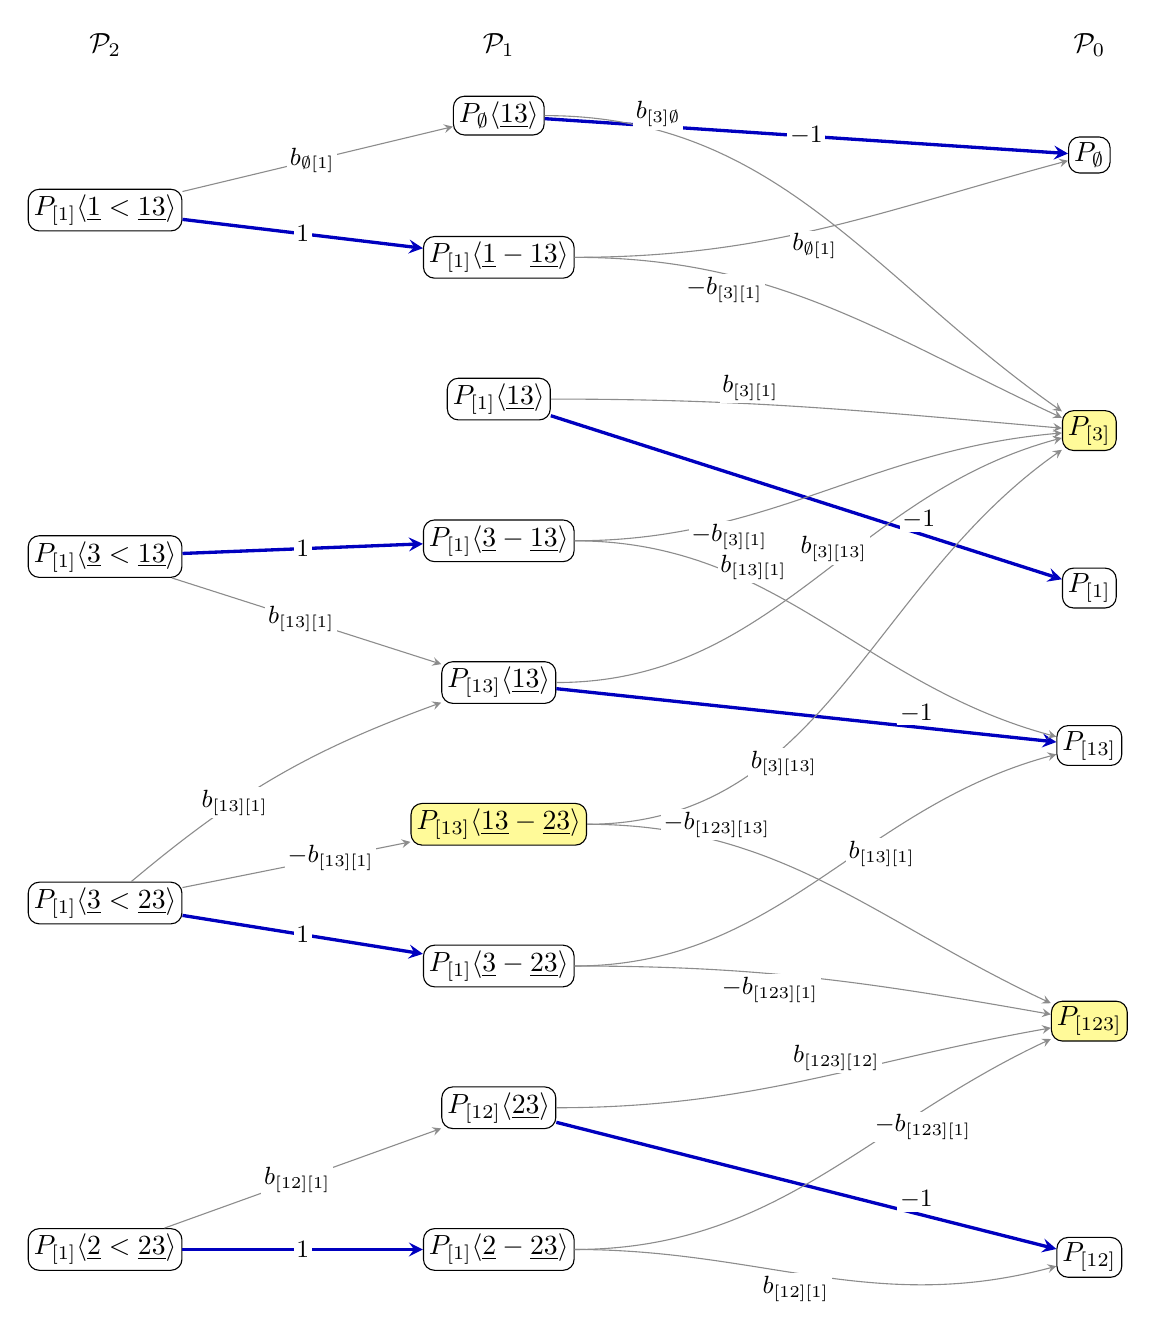
\begin{tikzpicture}[
  >=stealth,
  every node/.style={inner sep=2pt},
  summand/.style={draw,rounded corners,fill=white},
  critical/.style={draw,rounded corners,fill=yellow!40},
  match/.style={->,very thick,draw=blue!75!black},
  other/.style={->,draw=black!45},
  labl/.style={fill=white,inner sep=1pt,font=\small,text=black}
]

% Degree labels
\node[draw=none,font=\normalsize\bfseries] at (0,0.9) {$\mathcal P_2$};
\node[draw=none,font=\normalsize\bfseries] at (5,0.9) {$\mathcal P_1$};
\node[draw=none,font=\normalsize\bfseries] at (12.5,0.9) {$\mathcal P_0$};

% Degree two
\node[summand] (E1) at (0,-1.2)  {$P_{[1]}\langle\underline{1}<\underline{13}\rangle$};
\node[summand] (E2) at (0,-5.6)  {$P_{[1]}\langle\underline{3}<\underline{13}\rangle$};
\node[summand] (E3) at (0,-10.0) {$P_{[1]}\langle\underline{3}<\underline{23}\rangle$};
\node[summand] (E4) at (0,-14.4) {$P_{[1]}\langle\underline{2}<\underline{23}\rangle$};

% Degree one
\node[summand]  (Le)  at (5, 0.0)  {$P_{\emptyset}\langle\underline{13}\rangle$};
\node[summand]  (B1)  at (5,-1.8)  {$P_{[1]}\langle\underline{1}-\underline{13}\rangle$};
\node[summand]  (L1)  at (5,-3.6)  {$P_{[1]}\langle\underline{13}\rangle$};
\node[summand]  (B2)  at (5,-5.4)  {$P_{[1]}\langle\underline{3}-\underline{13}\rangle$};
\node[summand]  (L13) at (5,-7.2)  {$P_{[13]}\langle\underline{13}\rangle$};
\node[critical] (H13) at (5,-9.0)  {$P_{[13]}\langle\underline{13}-\underline{23}\rangle$};
\node[summand]  (B3)  at (5,-10.8) {$P_{[1]}\langle\underline{3}-\underline{23}\rangle$};
\node[summand]  (L12) at (5,-12.6) {$P_{[12]}\langle\underline{23}\rangle$};
\node[summand]  (B4)  at (5,-14.4) {$P_{[1]}\langle\underline{2}-\underline{23}\rangle$};

% Degree zero
\node[summand]  (Ue)   at (12.5,-0.5)  {$P_{\emptyset}$};
\node[critical] (U3)   at (12.5,-4.0)  {$P_{[3]}$};
\node[summand]  (U1)   at (12.5,-6.0)  {$P_{[1]}$};
\node[summand]  (U13)  at (12.5,-8.0)  {$P_{[13]}$};
\node[critical] (U123) at (12.5,-11.5) {$P_{[123]}$};
\node[summand]  (U12)  at (12.5,-14.5) {$P_{[12]}$};

% Matching arrows from degree two to degree one
\draw[match] (E1) -- node[labl] {$1$} (B1);
\draw[match] (E2) -- node[labl] {$1$} (B2);
\draw[match] (E3) -- node[labl] {$1$} (B3);
\draw[match] (E4) -- node[labl] {$1$} (B4);

% Remaining arrows from degree two to degree one
\draw[other] (E1) -- node[labl,pos=0.48] {$b_{\emptyset[1]}$} (Le);
\draw[other] (E2) -- node[labl,pos=0.48] {$b_{[13][1]}$} (L13);
\draw[other] (E3) to[bend left=10]
  node[labl,pos=0.35] {$b_{[13][1]}$} (L13);
\draw[other] (E3) -- node[labl,pos=0.65] {$-b_{[13][1]}$} (H13);
\draw[other] (E4) -- node[labl,pos=0.48] {$b_{[12][1]}$} (L12);

% Matching arrows from degree one to degree zero
\draw[match] (Le)  -- node[labl] {$-1$} (Ue);
\draw[match] (L1)  -- node[labl,pos=0.72,above] {$-1$} (U1);
\draw[match] (L13) -- node[labl,pos=0.72,above] {$-1$} (U13);
\draw[match] (L12) -- node[labl,pos=0.72,above] {$-1$} (U12);

% Remaining arrows from the B-parts
\draw[other] (B1) to[out=0,in=-165]
  node[labl,pos=0.48,below] {$b_{\emptyset[1]}$} (Ue);
\draw[other] (B1) to[out=0,in=155]
  node[labl,pos=0.28,below] {$-b_{[3][1]}$} (U3);

\draw[other] (B2) to[out=0,in=165]
  node[labl,pos=0.35,above] {$b_{[13][1]}$} (U13);
\draw[other] (B2) to[out=0,in=-175]
  node[labl,pos=0.30,below] {$-b_{[3][1]}$} (U3);

\draw[other] (B3) to[out=0,in=-165]
  node[labl,pos=0.65,below] {$b_{[13][1]}$} (U13);
\draw[other] (B3) to[out=0,in=170]
  node[labl,pos=0.40,below] {$-b_{[123][1]}$} (U123);

\draw[other] (B4) to[out=0,in=-165]
  node[labl,pos=0.45,below] {$b_{[12][1]}$} (U12);
\draw[other] (B4) to[out=0,in=-155]
  node[labl,pos=0.74,below] {$-b_{[123][1]}$} (U123);

% Remaining arrows from the L-parts
\draw[other] (Le)  to[out=0,in=145]
  node[labl,pos=0.18,above] {$b_{[3]\emptyset}$} (U3);
\draw[other] (L1)  to[out=0,in=175]
  node[labl,pos=0.38,above] {$b_{[3][1]}$} (U3);
\draw[other] (L13) to[out=0,in=-165]
  node[labl,pos=0.55,above] {$b_{[3][13]}$} (U3);
\draw[other] (L12) to[out=0,in=-170]
  node[labl,pos=0.57,above] {$b_{[123][12]}$} (U123);

% Arrows from the critical degree-one summand
\draw[other] (H13) to[out=0,in=-145]
  node[labl,pos=0.36,below] {$b_{[3][13]}$} (U3);
\draw[other] (H13) to[out=0,in=155]
  node[labl,pos=0.25,above] {$-b_{[123][13]}$} (U123);

\end{tikzpicture}
\caption{The weighted quiver after the $B\oplus H\oplus L$ change
of basis.}
\label{fig:morse-matching-change-of-basis}
\end{figure}

In Figure~\ref{fig:morse-matching-change-of-basis}, the thick blue arrows
form the Morse matching, the thin gray arrows are the remaining non-zero
matrix components of the differential, and the yellow vertices are
critical points. 

The two yellow-boxed summands $P_{[3]}$ and $P_{[123]}$
in Figure~\ref{fig:complex-picture} are precisely the degree-zero
terms of the resulting Morse complex.  Its degree-one term
is the copy of $P_{[13]}$ represented in the original basis by
$p^{(\underline{3}<\underline{13})}-p^{(\underline{3}<\underline{23})}$, for $p\in P_{[13]}$.
For the displayed choice of splitting, the remaining differential is
\[
 d_{\min,1}\colon P_{[13]}\longrightarrow P_{[3]}\oplus P_{[123]},
 \qquad
 p\longmapsto
 \bigl(b_{[3][13]}p,-b_{[123][13]}p\bigr).
\]
\end{eg}

\subsection{Projective dimension and Castelnuovo--Mumford regularity}
The formula for $\pdim I_X$ bears a striking resemblance to the characterisation of Castelnuovo--Mumford regularity by reduced homology:
\begin{align}
\pdim I_X
&=\max\{k\geq 0:\widetilde H_{k-1}(\Delta_Z)\neq 0 \text{ for some }Z\in L\}, \\
\operatorname{reg}\Bbbk[K]
&=\max\{k\geq 0:\widetilde H_{k-1}(\operatorname{lk}_K F)\neq 0 \text{ for some }F\in K\}. \label{eq:reg=non-vanishing homology}
\end{align}
Here $K$ is a finite simplicial complex, $\Bbbk[K]$ is its Stanley--Reisner ring and $\operatorname{reg}$ denotes the Castelnuovo--Mumford regularity (Definition \ref{def:SR ring}), and $\operatorname{lk}_K F$ is the link of $F$ in $K$ (see Definition \ref{def:link,face poset,sd}).  
For the equality \eqref{eq:reg=non-vanishing homology}, it is an application (Lemma \ref{lem:Hochshster easier}) of a more well-known Hochster's formula.
This motivates us to seek a complex $K$ for which we can associate to each $\Delta_Z$ a homologous link $\operatorname{lk}_K F$.  

We explain the idea of how to seek a suitable $K$.
First, the most natural choice of $K$ should be a refinement of $\D_X$ since we hope every $\Delta_Z$ can appear as a link (or at least homologous to it), and it seems to be the nicest case is to have $D_Z$ as a face.
Next, if we approach from the link side, then it seems natural to replace the link in \eqref{eq:reg=non-vanishing homology} by an order complex of a poset $\mathcal{F}_{K,F}$ constructed out of $(K,F)$, so that we get ourselves to align as close as possible to $\Delta_Z$. 
More precisely, we ask if there is a poset $\mathcal{F}_{K,F}$ such that $\widetilde{H}_k(\Delta(\mathcal{F}_{K,F}))\cong \widetilde{H}_k(\operatorname{lk}_KF)$ for all $k$ -- this is already available in the literature (see Lemma \ref{lem:munkres}), namely, by taking $\mathcal{F}_{K,F}$ to be the poset $\mathcal{F}^\times(\operatorname{lk}_KF)$ of non-empty faces of $\operatorname{lk}_K F$.

Now that we have order complexes of two different posets, we can then use order homotopy thoerem \cite[Theorem 10.11]{Bjo95} to see if their order complexes have the same reduced homology by just finding order-preserving maps.
Since we are looking at faces (i.e. sets) containing $F$, and we want $F=D_Z$, and we also want an order-preserving map from $\D_{X,>Z}$ to a face poset, these lead us to the following choice of $K$:
\[
\mathcal S_X:=\{S\subseteq P \mid S\subseteq D_T \text{ for some }D_T\in\mathcal D_X\} = \bigcup_{D_T\in \max \D_X} \mathbf{2}^{D_T},
\]
where $\mathbf{2}^U$ denotes the power set of $U$.  Indeed, a face in $\mathcal{S}_X$ containing some $D_Z$ tells us possible choices to extend $D_Z$ to a chain, which feels very close to what $\Delta_Z$ describes.
Our main result of this subsection is the following.

\begin{thm}\label{thm:pdim=reg}
Let $\Bbbk$ be a field, $\Sigma_{\mathcal{J}(P)}$ be the distance algebra associated to the lattice $\mathcal{J}(P)$ defined over $\Bbbk$.
Then, for any $X\in\mathcal{J}(P)$, we have
\[
\operatorname{pdim}_A I_X=\operatorname{reg}\Bbbk[\mathcal S_X].
\]
\end{thm}

In fact, the first step of the proof is to show that
$\widetilde H_r(\Delta_Z)\cong\widetilde H_r(\operatorname{lk}_{\mathcal S_X}D_Z)$ for all $r\ge -1$, which gives us $\pdim I_X\le \operatorname{reg} \Bbbk[\mathcal{S}_X]$.
To get the equality, the second step is to show that $\operatorname{lk}_{\mathcal S_X}F$ has zero reduced homology whenever $F\in\mathcal S_X\setminus\mathcal D_X$. 
Both steps use the fact that $\mathcal D_X$ is closed under intersection.

Before we dive into the proof, let us review some terminologies and results in algebraic topology.

\begin{dfn}\label{def:link,face poset,sd}
Let $K$ be a finite simplicial complex.  For a face $F\in K$, define its \defn{link} of $F$ in $K$ by
\[
\operatorname{lk}_K F:=\{G\subseteq V\setminus F:F\cup G\in K\}.
\]
Define the \defn{face poset} and the \defn{non-empty-face poset} of $K$ as
\[
\mathcal F(K):=\{\text{faces of }K\}, \quad \mathcal{F}^\times(K):=\mathcal{F}(K)\setminus\{\emptyset\},
\]
respectively, ordered by inclusion.  The \defn{barycentric subdivision} $\operatorname{sd}K$ of $K$ is the order complex of the non-empty-face poset of $K$.
\end{dfn}


\begin{lem}\label{lem:munkres}
There is an isomorphism of simplicial complexes
\[
\Delta\bigl(\mathcal F(K)_{>F}\bigr)
\cong\operatorname{sd}(\operatorname{lk}_K F).
\]
In particular, we have $\widetilde{H}_k(\operatorname{lk}_KF)\cong \widetilde{H}_k(\Delta(\mathcal{F}(K)_{>F}))$ for all $k\ge -1$.
\end{lem}
\begin{proof}
The first part is known in \cite[Lemma 15.3]{Mun84}; we can also obtain it using the poset isomorphism
\newcommand{\mapsfrom}{\mathrel{\reflectbox{$\mapsto$}}}
\[
\mathcal F(K)_{>F}:=\{F'\in K\mid F\subsetneq F'\} \rightarrow
\mathcal{F}^\times(\operatorname{lk}_K F),
\qquad F'\mapsto F'\setminus F, \text{ with inverse } F\cup H \mapsfrom  H.
\]
The second part follows from 
\[
\widetilde{H}_k(\operatorname{lk}_KF)\cong \widetilde{H}_k\big(\operatorname{sd}(\operatorname{lk}_KF)\big) \cong \widetilde{H}_k\big(\Delta(\mathcal{F}(K)_{>F})\big),
\]
where the first isomorphism uses the fact that barycentric subdivision preserves reduced homology \cite[Theorem 17.2]{Mun84}.
\end{proof}

As mentioned, we also need an order homotopy theorem, that is, a sufficient condition for two posets to have the same reduced homologies of their order complexes.

Let $f:Q\to Q'$ be an order-preserving maps between two finite posets $Q,Q'$.  Define, for all $k\ge 0$, a map $f_{\#,k}:C_k(\Delta(Q))\to C_k(\Delta(Q'))$ given by
\[
\langle x_0<\cdots<x_k\rangle \mapsto
\begin{cases}
\langle f(x_0)<\cdots<f(x_k)\rangle, & f(x_0),\ldots,f(x_k)\text{ are pairwise distinct},\\
0,&\text{otherwise}.
\end{cases}
\]
We also set $f_{\#,-1}=\id_{\Bbbk}$. 
Then $f_\#$ is a chain map on the chain complexes and their augmentations.

\begin{lem}\label{lem:order homotopy}
Let $f,g:Q\to Q'$ be order-preserving maps between finite posets, and suppose that $f(q)\leq g(q)$ for every $q\in Q$. 
These induce chain maps $f_\#, g_\#$ are chain homotopic.
\end{lem}
\begin{proof}
This is the chain complex version of \cite[Theorem 10.11]{Bjo95}; see also \cite[Theorem 13.3]{Mun84}.
We can verify it directly as follows.    
For $k\geq0$, define a map $h_k:C_k(\Delta(Q))\longrightarrow C_{k+1}(\Delta(Q'))$ by
\[
\langle x_0<\cdots<x_k\rangle\mapsto
\sum_{j=0}^k(-1)^j
\langle f(x_0)\leq\cdots\leq f(x_j)\leq g(x_j)\leq\cdots\leq g(x_k)\rangle.
\]
Every chain displayed on the right is weakly increasing, so to get well-defined map we interpret each summand containing repeated members as zero.  Set also $h_{-1}=0$.  Then it is routine to check that
\[
\partial_{k+1}^{Q'} h_k+h_{k-1}\partial_k^{Q} = g_{\#,k}-f_{\#,k},
\]
which gives the desire homotopy.
\end{proof}

Now we can start focusing on the setting of $\D_X$ and $\mathcal{S}_X$.

\begin{lem}\label{lem:face closure map}
The poset $\mathcal D_X$ is closed under intersections of non-empty finite families. The map
\[
c:\mathcal F(\mathcal S_X)\longrightarrow\mathcal D_X,\qquad
F\longmapsto\bigcap_{\substack{D_Y\in\max\mathcal D_X\\F\subseteq D_Y}}D_Y
\]
is well-defined, preserves inclusion, and satisfies $F\subseteq c(F)$.
\end{lem}

\begin{proof}
For $Y,Z\in\mathcal J(P)$, put
\[
T:=(X\cap Y)\cup(X\cap Z)\cup(Y\cap Z).
\]
The set $T$ is an ideal of $P$. Inside $X$, the elements of $D_Y\cap D_Z$ are those omitted by both $Y$ and $Z$; outside $X$, they are those contained in both. Hence
\[
D_Y\cap D_Z
=\bigl(X\setminus(Y\cup Z)\bigr)\cup\bigl((Y\cap Z)\setminus X\bigr)
=X\SDiff T=D_T.
\]
Closure under intersections of non-empty finite families follows by induction.

Every $F\in\mathcal S_X$ is contained in a facet, so the family defining $c(F)$ is non-empty. Closure under intersections gives $c(F)\in\mathcal D_X$, and every set in the intersection contains $F$. If $F\subseteq G$, the family of facets containing $G$ is contained in the family containing $F$. Therefore $c(F)\subseteq c(G)$.
\end{proof}


\begin{lem}\label{lem:H(Delta Z)=H(lk DZ)}
For every $Z\in\mathcal J(P)$ and every $k\geq-1$,
\[
\widetilde H_k(\Delta_Z)\cong
\widetilde H_k\bigl(\operatorname{lk}_{\mathcal S_X}(D_Z)\bigr).
\]
\end{lem}

\begin{proof}
The set $D_Z$ is a face of $\mathcal S_X$. Consider the order-preserving maps
\[
j_Z:\mathcal D_{X,>D_Z}\longrightarrow\mathcal F(\mathcal S_X)_{>D_Z},
\qquad D_T\longmapsto D_T,
\]
\[
c_Z:\mathcal F(\mathcal S_X)_{>D_Z}\longrightarrow\mathcal D_{X,>D_Z},
\qquad F\longmapsto c(F).
\]
The map $c_Z$ is well-defined because $D_Z<F\subseteq c(F)$ by Lemma \ref{lem:face closure map}. Moreover, we have
\[
D_T\subset c_Zj_Z(D_T), \text{ for all $D_T\in\D_{X,>D_Z}$ and }
F\subseteq  j_Zc_Z \text{ for all $F\in\mathcal{F}(\mathcal{S}_X)_{>D_Z}$.}
\]
Hence, Lemma \ref{lem:order homotopy} says that $j_{Z,\#}$ and $c_{Z,\#}$ are chain homotopy inverses. Thus, the order complexes of $\mathcal D_{X,>D_Z}$ and $\mathcal F(\mathcal S_X)_{>D_Z}$ have isomorphic reduced homology.
Now applies Lemma \ref{lem:munkres} and get that
\[
\widetilde{H}_k(\Delta_Z) 
\cong \widetilde{H}_k(\Delta\big(\mathcal{F}(\mathcal{S}_X)_{D_Z}\big)) 
\cong \widetilde{H}_k(\operatorname{lk}_{\mathcal{S}_X}{D_Z}) \text{ for all }k\ge -1,
\]
which proves the claim.
\end{proof}

Now we need to look at the reduce homologies of links of faces $F\in \mathcal{S}_X\setminus \D_X$.

Recall that a simplicial complex $K$ is a \defn{cone with vertex $p$} if $p\in V(K)$ and $\sigma\cup\{p\}\in K$ for every $\sigma\in K$.  A cone has zero reduced homology. Indeed, send $1\in \Bbbk = C_{-1}(K)$ to $\langle p\rangle$, and order its vertices with $p$ be the minimum, then the map
\[
\langle v_0< \ldots < v_k\rangle \mapsto \begin{cases}
    \langle p < v_0 < \ldots < v_k\rangle, & p\neq v_i \text{ for all }0\le i\le k,\\
    0, & \text{otherwise}
\end{cases} 
\]
defines a contraction of $C_\bullet(K)$.

\begin{lem}\label{lem:bad face has 0 homology link}
If $F\in\mathcal S_X$ and $F\notin\mathcal D_X$, then
$\operatorname{lk}_{\mathcal S_X}(F)$ is a cone. In particular,
\[
\widetilde H_i\bigl(\operatorname{lk}_{\mathcal S_X}(F)\bigr)=0
\qquad\text{for every }i.
\]
\end{lem}

\begin{proof}
Since $c(F)\in\mathcal D_X$ and $F\notin\mathcal D_X$, the inclusion $F\subseteq c(F)$ is strict. Choose $p\in c(F)\setminus F$.

For $G\in\operatorname{lk}_{\mathcal S_X}(F)$, choose a facet $D_Y$ containing $F\cup G$. The definition of $c(F)$ gives $p\in D_Y$, so $F\cup G\cup\{p\}\subseteq D_Y$. Since $p\notin F$, it follows that $G\cup\{p\}\in\operatorname{lk}_{\mathcal S_X}(F)$. Thus the link is a cone with vertex $p$.
\end{proof}

Let us review the necessary background we need about Stanley--Reisner ring before proving Theorem \ref{thm:pdim=reg}.

\begin{dfn}\label{def:SR ring}
Let $K$ be a finite simplicial complex and put $S_K:=\Bbbk[x_v\mid v\in V(K)]$, with $\deg x_v=1$. Its \emph{Stanley--Reisner ideal} and \emph{Stanley--Reisner ring} are
\[
I(K):=\left(\prod_{v\in F}x_v\ \middle|\ F\subseteq V(K),\ F\notin K\right),
\qquad \Bbbk[K]:=S_K/I(K).
\]
Thus a product of distinct variables is non-zero in $\Bbbk[K]$ precisely when its support is a face of $K$.

Write the $i$-th term of the minimal graded free resolution of $\Bbbk[K]$ over $S_K$ as $\bigoplus_j S_K(-j)^{\oplus \beta_{i,j}}$, where $(-j)$ denotes the grading shift so that $1\in S_K(-j)$ is in degree $j$. The \emph{Castelnuovo--Mumford regularity} is
\[
\operatorname{reg}\Bbbk[K]:=\max\{j-i\mid\beta_{i,j}\neq0\}.
\]
For $K=\{\emptyset\}$, set $S_K=\Bbbk$, so $\operatorname{reg}\Bbbk[K]=0$.
\end{dfn}

\begin{lem}\label{lem:Hochshster easier}
For every finite simplicial complex $K$,
\[
\operatorname{reg}\Bbbk[K]
=\max\{k\geq0\mid\widetilde H_{k-1}(\operatorname{lk}_K(F))\neq0
\text{ for some }F\in K\}.
\]
\end{lem}
\begin{proof}
This is the link formulation of Hochster's formula stated in \cite[Lemma 2.21]{Ha14}, but it assumes the ground ring $\Bbbk$ is an infinite field. 
This can be overcome for finite field $\Bbbk$ by extending scalars to $\Bbbk(t)$ since simplicial homology commutes with field extension, and a minimal graded free resolution remains minimal after field extension -- so it preserves the graded Betti number $\beta_{i,j}$ and hence the regularity.    
\end{proof}


\begin{proof}[Proof of Theorem \ref{thm:pdim=reg}]
This follows from
\begin{align*}
\operatorname{pdim}_A I_X
&=\max\{k\geq0\mid\widetilde H_{k-1}(\Delta_Z)\neq0
             \text{ for some }Z\in\mathcal J(P)\}\\
&=\max\{k\geq0\mid\widetilde H_{k-1}(\operatorname{lk}_{\mathcal S_X}(F))\neq0
             \text{ for some }F\in\mathcal S_X\}\\
&=\operatorname{reg}\Bbbk[\mathcal S_X],
\end{align*}
where the first equality follows from Corollary \ref{cor:SigmaJ(P) is IG} and the last equality follows from Lemma \ref{lem:Hochshster easier}.
For the middle equality, we get $\le$ from Lemma \ref{lem:H(Delta Z)=H(lk DZ)}, whereas $\ge$ follows from Lemma \ref{lem:bad face has 0 homology link}.
\end{proof}


%%%%%%%%%%%%%%%%%%%%%%%%%%%%%%%%%%%%%%%%%%%%%%%%%%%%%%%%%%%%%
%%%%%%%%%%%%%%%%%%%%%%%%%%%%%%%%%%%%%%%%%%%%%%%%%%%%%%%%%%%%%

\section{Multiplicity in low degrees}
\label{sec:low-degree-multiplicity}

We now investigate further properties of the minimal projective resolution constructed above.
Recall that for a finitely generated projective right $A$-module $Q$, by the Krull--Schmidt theorem, it has a decomposition
\[
 Q\cong\bigoplus_{Z\in\mathcal J(P)}P_Z^{\oplus m_Z}.
\]
The integer $m_Z$ is the \defn{multiplicity} of $P_Z$ in $Q$, denoted $\bigl[Q:P_Z\bigr]$.  We call $Q$ \defn{multiplicity-free} if $\bigl[Q:P_Z\bigr]\leq1$ for every $Z\in\mathcal J(P)$.

For the minimal resolution of $I_X$ constructed in Theorem~\ref{thm:minimal-resolution}, equation~\eqref{eq:minimal-terms} gives
\begin{equation*}
 \bigl[\mathcal P_{\min,k}:P_Z\bigr]
 =\widetilde\beta_{Z,k}
 =\dim_{\Bbbk}\widetilde H_{k-1}(\Delta_Z).
\end{equation*}
In the following subsections, we see some possible behavior exhibit by these multiplicities.

\subsection{Multiplicity-free in degree zero and one}
\label{subsec:multi-free deg 0 1}
In degrees zero and one, the topology of $\Delta_Z$ is sufficiently restricted to give the following multiplicity-free results.

\begin{prop}\label{prop:low-degree-multiplicity}
The projective modules $\mathcal P_{\min,0}$ and $\mathcal P_{\min,1}$ are multiplicity-free.
\end{prop}

\begin{proof}
For $k=0$, the multiplicity of $P_Z$ is $\dim_{\Bbbk}\widetilde H_{-1}(\Delta_Z)$, which is $1$ when $\Delta_Z=\emptyset$ and is $0$ otherwise.

Now consider $k=1$.  We have
\begin{equation*}
 \widetilde\beta_{Z,1}
 =\dim_{\Bbbk}\widetilde H_0(\Delta_Z)
 =\#\{\text{connected components of the $1$-skeleton of }\Delta_Z\}-1.
\end{equation*}
The $1$-skeleton of $\Delta_Z$ is a graph whose  elements are $D_Y\in\mathcal D_{X,>Z}$, and two vertices $D_Y,D_{Y'}$ are adjacent precisely when they are comparable.
It then suffices to show that the $1$-skeleton of $\Delta_Z$ has at most two connected components.
Note that if $\mathcal D_{X,>Z}=\emptyset$, then the $1$-skeleton of $\Delta_Z$ is just the point $\emptyset$ and $\widetilde H_0(\Delta_Z)=0$.  

Every vertex $D_Y\in \mathcal{D}_{X,>Z}$ falls into one of the three cases (a) $Y\subsetneq Z$, (b) $Z\subsetneq Y$, or (c) $Y$ and $Z$ are incomparable.  In case (a), if $Y,Y'\subsetneq Z$, then $Y\cap Y'$ is an order ideal and
\[
 D_Y\subseteq D_{Y\cap Y'},\qquad
 D_{Y'}\subseteq D_{Y\cap Y'},\qquad
 D_Z\subsetneq D_{Y\cap Y'}.
\]
Thus all vertices in case (a) lie in one connected component.  Similarly, if $Z\subsetneq Y,Y'$, then $Y\cup Y'$ is an order ideal and
\[
 D_Y\subseteq D_{Y\cup Y'},\qquad
 D_{Y'}\subseteq D_{Y\cup Y'},\qquad
 D_Z\subsetneq D_{Y\cup Y'}.
\]
Thus all vertices in case (b) lie in one connected component.

Finally, suppose that $Y$ and $Z$ are incomparable.  Then
\[
 D_{Y\cap Z}=D_Z\sqcup(Z\setminus Y),\qquad
 D_{Y\cup Z}=D_Z\sqcup(Y\setminus Z).
\]
Both are vertices of the $1$-skeleton and are comparable with $D_Y$; the first corresponds to an order ideal properly contained in $Z$, whereas the second corresponds to one properly containing $Z$.  Consequently, any $Y$ incomparable with $Z$ belongs to one of the two components described.
\end{proof}

%%%%%%%%%%%%%%%%%%%%%%%%%%%%%%%%%%%%%%%%%%%%%%%%%%%%%%%%%%%%%%%%%%%%%%%%%%%
\subsection{Higher multiplicities via independence complexes}
\label{subsec:higher-multiplicities}

In contrast to the behavior in degree $0$ and $1$, we demonstrate that multiplicities can be arbitrary large in higher degrees already when $P$ is a height-two poset.

Let $B=(X\sqcup Y,E)$ be a (finite) bipartite graph so we can regard $E\subseteq X\times Y$.  Specifying such a $B$ is equivalent to specifying a height-two poset, namely, the corresponding poset is given by $(P_B=X\sqcup Y, \le)$ with 
\[
 x<y
 \quad\Leftrightarrow\quad
 \{x,y\}\in E
 \qquad(x\in X,\ y\in Y),
\]
and no other strict relations.  Conversely, the Hasse diagram of a height two poset $(P=X\sqcup Y, \le)$, where $X$ is of height $0$ and $Y$ is of height $1$, is precisely the bipartite graph $B$ with $P_B=P$.

A subset $\sigma\subseteq V(B)$ is \defn{independent} if no two vertices of $\sigma$ are joined by an edge of $B$.  The \defn{independence complex} $\Ind(B)$ is the simplicial complex on $V(B)$ whose faces are the independent subsets of $B$.

\old{
For a finite simplicial complex $K$, let $\mathcal F(K)$ be the poset of all faces of $K$, including the empty face, ordered by inclusion, and set $\mathcal F^\times(K):=\mathcal F(K)\setminus\{\emptyset\}$.  The order complex of the poset $\mathcal{F}^\times(K)$ is called \defn{barycentric subdivision} $\sd K:=\Delta(\mathcal{F}^\times(K))$ of $K$. 
Note that the geometric realizations $|\sd K|$ and $|K|$ are homeomorphic; in particular, $K$ and $\sd K$ have the same reduced homology.}

\begin{prop}\label{prop:height-two-independence}
For a bipartite graph $B=(X\sqcup Y,E)$, the poset $\mathcal F\bigl(\Ind(B)\bigr)$ is the same as $\D_X$ associated to the height-two poset $P_B$. 
In particular, we have $\sd\Ind(B)=\Delta(\D_X\setminus\{\emptyset\}) = \Delta_X$,
and hence
\[
 [\mathcal P_{\min,k}:P_X] = \beta_{X,k} = \widetilde H_{k-1}(\Delta_X)
 \cong\widetilde H_{k-1}(\Ind(B))
 \text{ for all } k\ge 0.
\]
\end{prop}

\begin{proof}
Fix $T\in \mathcal{J}(P_B)$.  We show that $D_T$ is an independent set of $B$.  Indeed, note that $D_T=(X\setminus T)\sqcup(T\cap Y)$, so if, on the contrary, $x\in X\setminus T$ and $y\in T\cap Y$ were adjacent in $B$, then $x<y$ in $P_B$.  But $T$ being an order ideal implies that $x\in T$, a contradiction.

Conversely, let $U$ be an independent set of $B$, we claim that $T_U:=\bigl(X\setminus(U\cap X)\bigr)\cup(U\cap Y)\in \mathcal{J}(P_B)$.  Indeed, if $y\in U\cap y$ and $x<y$ in $P_B$, then independence gives $x\notin U$, so $x\in T_U$.  
Since \[
D_{T_U} =  D_{X\setminus (U\cap X)}  \cup  D_{U\cap Y}= (U\cap X) \cup (U\cap Y) = U,
\]
we get that $\mathcal F(\Ind(B))$ are the same collection of subsets as $\D_X$.  Since both posets use inclusion order, they are the same poset.

The last assertion follows by noticing that $D_X=\emptyset$.
\end{proof}

By Proposition~\ref{prop:height-two-independence}, a bipartite graph $B$ with $\Ind(B)$ that has reduced homology of dimension greater than one gives a non-multiplicity-free term we desired.

\begin{eg}
Consider a bipartition $B$ of $C_6\sqcup K_2$ given by
\[
 X=\{1,2,3,4\},
 \qquad
 Y=\{5,6,7,8\},
\]
so that $P_B$ is of the form:
\begin{center}
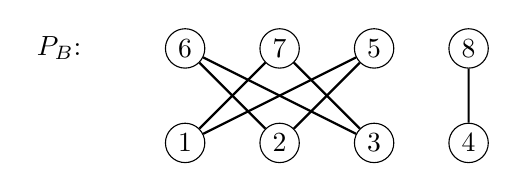
\begin{tikzpicture}[scale=0.8,
  vertex/.style={
    circle,
    draw,
    fill=white,
    inner sep=0pt,
    minimum size=5mm
  }
]
 \node at (-2,1.5) {$P_B$:};\node[vertex] (1) at (0,0) {1};
  \node[vertex] (2) at (1.5,0) {2};
  \node[vertex] (3) at (3,0) {3};
  \node[vertex] (4) at (4.5,0) {4};
  \node[vertex] (5) at (3,1.5) {5};
  \node[vertex] (6) at (0,1.5) {6};
  \node[vertex] (7) at (1.5,1.5) {7};
  \node[vertex] (8) at (4.5,1.5) {8};
  \draw[thick] (5)--(1);
  \draw[thick] (5)--(2);
  \draw[thick] (6)--(2);
  \draw[thick] (6)--(3);
  \draw[thick] (7)--(3);
  \draw[thick] (7)--(1);
  \draw[thick] (8)--(4);
\end{tikzpicture}
\end{center}
We can draw $\Ind(C_6)$ as follows, where the 2-simplices are filled triangles $\{1,2,3\}$ and $\{5,6,7\}$, and three additional maximal faces $\{1,6\}, \{2,7\}, \{3,5\}$.
\begin{center}
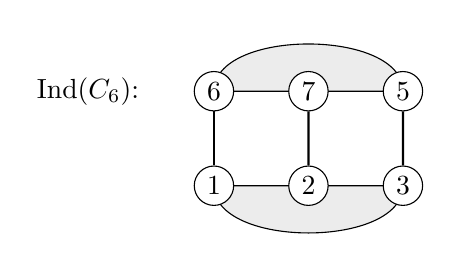
\begin{tikzpicture}[scale=0.8,
  vertex/.style={
    circle,
    draw,
    fill=white,
    inner sep=0pt,
    minimum size=5mm
  }
]  
\node at (-2,1.5) {$\Ind(C_6)$:};
% Filled 2-simplices, drawn behind the vertices.
  \path[draw,fill=gray!15]
    (0,0) -- (1.5,0) -- (3,0)
    .. controls +(0,-1) and +(0,-1) .. (0,0)
    -- cycle;
  \path[draw,fill=gray!15]
    (0,1.5) -- (1.5,1.5) -- (3,1.5)
    .. controls +(0,1) and +(0,1) .. (0,1.5)
    -- cycle;
\node[vertex] (1) at (0,0) {1};
  \node[vertex] (2) at (1.5,0) {2};
  \node[vertex] (3) at (3,0) {3};
  \node[vertex] (5) at (3,1.5) {5};
  \node[vertex] (6) at (0,1.5) {6};
  \node[vertex] (7) at (1.5,1.5) {7};
  \draw[thick] (6)--(1);
  \draw[thick] (7)--(2);
  \draw[thick] (5)--(3);
\end{tikzpicture}
\end{center}
Contracting the two $2$-simplices yields a graph with two vertices joined by three edges, which means that we have homotopic equivalent space $|\Ind(C_6)|\simeq S^1\vee S^1$, where $\vee$ here denotes the wedge sum.  Also, we have $|\Ind(K_2)|=S^0$.  

Note that an independent set of a disjoint union $G\sqcup H$ is the union of an independent set of $G$ and one of $H$, i.e. $\Ind(G\sqcup H)=\Ind(G)\ast \Ind(H)$, where $\ast$ denotes the simplicial join (faces are the union of those in the two components).  Since joining with $S^0$ is homotopic to taking the suspension $\Sigma(-)$, and suspension preserves wedge sums, we get a homotopy equivalence
\begin{align*}
 |\Ind(B)|
 &=|\Ind(C_6)*\Ind(K_2)|\\
 &\simeq(S^1\vee S^1)*S^0
 \simeq\Sigma(S^1\vee S^1)\simeq S^2\vee S^2.
\end{align*}
Hence, for $k\ge 0$, we have
\[
\widetilde{H}_k(\Ind(B)) \cong  \widetilde{H}_k(S^2\vee S^2) \cong \widetilde{H}_k(S^2)^{\oplus 2} = \begin{cases}
    \Bbbk^{\oplus 2}, & k=2, \\ 0, & \text{otherwise.}
\end{cases}
\]
In particular, we have $[\mathcal{P}_{\min,k+1}:P_X]=2$, i.e. $\mathcal P_{\min,3}$ is not multiplicity-free.
\end{eg}

In general, we can wedge more spheres to get arbitrary multiplicity in reduced homology.

\begin{eg}\label{eg:complexes-with-arbitrary-homology}
%\comment{don't need $\widetilde{H}_{0}$ since multi-free there}
For $m\geq1$ and $k\ge 2$, take a finite triangulation of $K=\bigvee_{j=1}^{m}S^{k-1}$.  Then $\widetilde H_{k-1}(K)\cong\Bbbk^m$.
\end{eg}

The final ingredient we need is the following realization theorem.

\begin{thm}\textnormal{(\cite[Proposition~6.2]{NR09})}
\label{thm:nagel-reiner}
For every finite simplicial complex $K$, there exists a finite bipartite graph $B_K$ such that $\Ind(B_K)\simeq\Sigma K$.
\end{thm}


\begin{cor}\label{cor:arbitrary-higher-multiplicities}
For every $k\geq2$ and every $m\geq1$, there exist a finite height-two poset $P$ and an order ideal $X\in\mathcal J(P)$ such that the multiplicity $[\mathcal{P}_{\min,k}:P_X]=m$ in the degree $k$ term of any minimal projective resolution $\mathcal{P}_{\min,\bullet}$ of the $\Sigma_{\mathcal{J}(P)}$-module $I_X$.
\end{cor}

\begin{proof}
Take $K=\bigvee_{j=1}^m S^{k-1}$, then we get that $\dim_{\Bbbk}\widetilde H_{k-1}(K)=m$ as seen in Example~\ref{eg:complexes-with-arbitrary-homology}.  Let $B_K=X \sqcup Y$ be the bipartite graph guaranteed by Theorem~\ref{thm:nagel-reiner} and take $P=P_{B_K}$, then the claim follows from Proposition~\ref{prop:height-two-independence}.
\end{proof}


\appendix

\section{A simplicial construction for thin modules}
\label{app:thin-modules}

The projective resolution in Section~\ref{sec:candidate-resolution} is an instance of the simplicial replacement (bar construction of \cite[Definition 4.2.1]{Rie14}) of a diagram of projective modules.  This explains why it looks very much like an economoical reformulation of bar construction.  For some modules, this construction always gives a complex of projectives, although the complex need not be exact.

Let $A=\Bbbk Q/I$ be a basic finite-dimensional bound-quiver algebra, and let $M$ be a \defn{thin} right $A$-module, i.e. $\dim_{\Bbbk}Me_i\leq1$ for every $i\in Q_0$.  Let $Q_M$ be the subquiver of $Q$ whose vertices are
\[
(Q_M)_0:=\{i\in Q_0\mid Me_i\neq0\}
\]
and whose arrows are those $a:i\to j$ for which right multiplication induces a non-zero map $Me_i\to Me_j$.  The key assumption we need is that non-zero vectors $m_i\in Me_i$ can be chosen so that
\begin{equation}
m_i a=m_j
\qquad
\text{for every arrow $a:i\to j$ in $Q_M$}.
\label{eq:thin-normalized-basis}
\end{equation}

The quiver $Q_M$ is acyclic.  Indeed, if it contained an oriented cycle, then \eqref{eq:thin-normalized-basis} would imply that every positive power of this cycle acts non-trivially on one of the vectors $m_i$.  This contradicts the admissibility of $I$, since every sufficiently long path belongs to $I$.

For every $i\in(Q_M)_0$, let
\[
\pi_i\colon P_i=e_iA\longrightarrow M
\]
be the homomorphism determined by $\pi_i(e_i)=m_i$.  Since each non-zero space $Me_i$ is spanned by $m_i$, these maps give a surjection
\begin{equation}\label{eq: pi to M}
\pi:=\bigl(\pi_i\bigr)_{i\in(Q_M)_0}\colon
\bigoplus_{i\in(Q_M)_0}P_i\longrightarrow M.
\end{equation}

Consider the small category $\mathcal C_M$ associated to $M$ given by taking the quotient of the opposite path category of $Q_M$ by the ideal that identifies paths inducing the same homomorphism between projective modules.  
For clarity, we can write out this definition explicitly as follows.  We take $(Q_M)_0$ as the objects of $\mathcal{C}_M$.  
Recall that for each path $p:j\to i$ on $Q_M$, we have a homomorphism $\mu_p:P_i\to P_j$ given by $x\mapsto px$.
The morphisms in $\mathcal{C}_M(i,j)$ are these $\mu_p$ where two paths determine the same morphism if they induce the same homomorphism.  In particular, the identity of $i$ is $\mu_{e_i}$.
Composition is determined by $\mu_q\mu_p=\mu_{qp}$ whenever $p:j\to i$ and $q:k\to j$.

Define a functor
\begin{equation*}
F_M\colon\mathcal C_M\longrightarrow\proj A,
\qquad
i\longmapsto P_i,
\qquad
\mu_p\longmapsto\mu_p.
\end{equation*}
If $\mu_p:i\to j$ is induced by a path $p:j\to i$, then \eqref{eq:thin-normalized-basis} gives $m_jp=m_i$.  Consequently, $\pi_j\mu_p=\pi_i$, so the homomorphisms $\pi_i$ form a cocone over $F_M$ with vertex $M$, and so there is a surjection induced by $\pi$ of \eqref{eq: pi to M}
\[
\colim_{\mathcal{C}_M} F_M\cong  \Big(\bigoplus_{i\in \mathcal{C}_M} P_i \Big) / \sum_{\substack{p:i\to j\\ m\in P_i}} (m^{(i)} - F_M(p)(m)^{(j)}) A \twoheadrightarrow M.
\]
If $M$ is additionally faithful, then this become an isomorphism.

For $k\geq0$, let $N_k(\mathcal C_M)$ be the set of composable strings of $k$ non-identity morphisms
\begin{equation*}
\sigma_\ast=
\bigl(
i_0\xrightarrow{f_1}i_1\xrightarrow{f_2}\cdots
\xrightarrow{f_k}i_k
\bigr).
\end{equation*}
In particular, $N_0(\mathcal C_M)$ is the object set of $\mathcal C_M$.  For $0\leq r\leq k$, write $\sigma_\ast^{\widehat r}$ for the string obtained by deleting $i_r$; when $0<r<k$, the adjacent morphisms $f_r$ and $f_{r+1}$ are replaced by their composite.

Define
\begin{equation*}
\mathcal P_k(M):=
\bigoplus_{\sigma_\ast\in N_k(\mathcal C_M)}
F_M(i_0)^{(\sigma_\ast)}.
\end{equation*}
Here \(F_M(i_0)^{(\sigma_\ast)}\) denotes a labelled copy of \(F_M(i_0)=P_{i_0}\).  For $k>0$, define
\[
d_k\colon\mathcal P_k(M)\longrightarrow\mathcal P_{k-1}(M)
\]
by
\begin{equation*}
d_k\bigl(x^{(\sigma_\ast)}\bigr)
:=
\bigl(F_M(f_1)(x)\bigr)^{(\sigma_\ast^{\widehat0})}
+\sum_{r=1}^k(-1)^r
x^{(\sigma_\ast^{\widehat r})}.
\end{equation*}
Thus the zeroth face changes the initial projective through $F_M(f_1)$, while every other face acts as the identity on the initial projective.

\begin{prop}\label{prop:cpx from module}
For a thin $A$-module $M$, taking $d_0:=\pi$ yields a complex of $A$-modules
\begin{equation*}
\cdots\longrightarrow\mathcal P_2(M)
\xrightarrow{d_2}\mathcal P_1(M)
\xrightarrow{d_1}\mathcal P_0(M)
\xrightarrow{d_0}M\to 0,
\end{equation*}
which is exact at $\mathcal{P}_0(M)$ when $M$ is faithful.
\end{prop}

\begin{proof}
For a string $\sigma_\ast$ and $0\leq r\leq k$, let $\varepsilon_r^{\sigma_\ast}$ be the homomorphism defines analogous to \eqref{eq:face map}.  The zeroth face is induced by $F_M(f_1)$, while every other face is the identity map between the corresponding labelled copies of $F_M(i_0)$.  Functoriality of $F_M$ gives the simplicial identities
\begin{equation*}
\varepsilon_i^{\sigma_\ast^{\widehat j}}
\varepsilon_j^{\sigma_\ast}
=
\varepsilon_{j-1}^{\sigma_\ast^{\widehat i}}
\varepsilon_i^{\sigma_\ast}
\qquad
(0\leq i<j\leq k).
\end{equation*}
The only identity involving two non-identity homomorphisms is the one obtained by deleting $i_0$ and $i_1$, and it follows from $F_M(f_2)F_M(f_1)=F_M(f_2f_1)$.  For $0\leq i<j\leq k$, the equal composites
$\varepsilon_i^{\sigma_\ast^{\widehat j}}\varepsilon_j^{\sigma_\ast}$
and $\varepsilon_{j-1}^{\sigma_\ast^{\widehat i}}\varepsilon_i^{\sigma_\ast}$
occur in $d_{k-1}d_k$ with coefficients $(-1)^{i+j}$ and $(-1)^{i+j-1}$, respectively. Hence $d_{k-1}d_k=0$ for $k\geq2$.

For a morphism $f:i_0\to i_1$ and $x\in P_{i_0}$, the the equality $\pi_{i_1}\circ F_M(f)=\pi_{i_0}$ gives
\[
d_0d_1\bigl(x^{(f)}\bigr)
=
\pi_{i_1}F_M(f)(x)-\pi_{i_0}(x)
=
0.
\]
Hence the displayed sequence is a complex.
\end{proof}

\begin{eg}\label{eg:DX is C_IX}
For $A=\Sigma_{\mathcal J(P)}$ and $M=I_X$, choose $m_Y\in I_Xe_Y$ to be the functional dual to $b_{YX}$.  Then $\mathcal C_{I_X}$ can be identified with the poset category $\D_X$: there is a non-identity morphism $Z\to T$ precisely when $D_Z<D_T$, and this morphism is represented by
\[
\mu_{T,Z}\colon P_Z\longrightarrow P_T,
\qquad
p\longmapsto b_{TZ}p.
\]    
The set $N_k(\mathcal{C}_M)$ becomes the $k$-chains in $\Delta(\D_X)$.
Note that $I_X$ is thin and faithful.
\end{eg}

\begin{eg}
For a simple module $S_i$, the category $\mathcal C_{S_i}$ has only the object $i$ and its identity morphism.  
Hence $\mathcal P_0(S_i)=P_i$ and $\mathcal P_k(S_i)=0$ for $k>0$, so the construction reduces to the projective cover $P_i\to S_i$.  It is a projective resolution only when $S_i$ is itself projective.  This shows how non-faithfulness yields non-exactness of $\mathcal{P}_\bullet$.
\end{eg}

Now we relate $\mathcal P_\bullet(M)$ to the two-sided simplicial bar construction used in \cite[Definition 4.2.1]{Rie14}; we note that this does not really give an alternative proof of Proposition \ref{prop:cpx from module} but rather the proof above demonstrates exactly the reason why the simplicial bar complex yields a complex in a certain special case.  We summarise the translation of setting as follows.

\begin{center}
\begin{tabular}{p{0.28\textwidth}p{0.64\textwidth}}
\hline
Bar construction setting & Our $\mathcal{C}_M$ setting\\
\hline
$\mathcal D$ & $\mathcal C_M$\\[4pt]
$\mathcal M$ & $s(\operatorname{Mod}A)$, the category of simplicial right $A$-modules.\\[4pt]
$F:\mathcal D\to\mathcal M$ & The composite $c\circ F_M$, where $F_M:\mathcal C_M\to\operatorname{proj}A$ and $c$ regards an ordinary module as a constant simplicial module.\\[4pt]
$G:\mathcal D^{\mathrm{op}}\to\mathrm{sSet}$ & The constant functor $G=*$ with value in $\ast\in \mathrm{sSet}$.\\[4pt]
$\vec d:[k]\to \mathcal D$ & A string $\sigma_\ast=(i_0\xrightarrow{f_1}\cdots\xrightarrow{f_k}i_k)$, but allowing identity morphisms.\\[4pt]
$Gd_k\otimes Fd_0$ & $*\otimes cF_M(i_0)\cong cF_M(i_0)$;\footnotemark\\[4pt]
$B_k(G,\mathcal D,F)$ & The constant simplicial module associated to $\bigoplus_{\sigma_\ast}F_M(i_0)$.\\[4pt]
Face maps & Our homomorphisms $\varepsilon_r^{\sigma_\ast}$; their alternating sum gives $d_k$.\\[4pt]
Degeneracy maps & The homomorphisms inserting identity morphisms into $\sigma_\ast$.\\
%[4pt]Normalized chain complex & $\mathcal P_\bullet(M)$, obtained by quotienting out the summands indexed by strings containing identity morphisms.\\
\hline
\end{tabular}
\end{center}
 \footnotetext{The $\otimes$ on the left is the simplicial tensoring, not tensor product of modules.}

\medskip

Let us explain the translation of $\mathcal M$ and $F$ now.
Recall that a simplicial right $A$-module is a functor $\Delta^{\mathrm{op}}\to\operatorname{Mod}A$, where $\Delta$ is the category of finite non-empty totally ordered sets $[n]=\{0<\ldots<n\}$ and order-preserving maps; roughly speaking, it is a sequence $\{M_k\}_{k\ge 0}$ of right $A$-modules (where \emph{degree $k$ term} $M_k$ is the functor evaluated at $[k]$) equipped with homomorphisms that delete or repeat positions, satisfying compatibility identities.  Every right $A$-module $N$ determines a \emph{constant simplicial module} $cN$, with $(cN)_k = N$ for all $k\ge 0$ and all structure maps are $\id_N$. We take
\[
\mathcal M=s(\operatorname{Mod}A),\qquad F=c\circ F_M:\mathcal C_M\longrightarrow s(\operatorname{Mod}A),
\]
where the inclusion $\operatorname{proj}A\hookrightarrow\operatorname{Mod}A$ is understood. Thus, we have $F(i)=cP_i$ for each $i\in \mathcal{C}_M=Q_M$.

Next, we unfold the definition of the simplicial bar construction to see how (the modules underlying) $\mathcal{P}_\bullet$ shows up in it.
Writing out the evaluation of a string $\vec d:[k]\to \D$ yields a sequence $d_0\xrightarrow{f_1} d_1 \xrightarrow{f_2} \cdots \xrightarrow{f_k} d_k$.  These $d_j$'s are our $i_j\in Q_M$, and so with the chosen $F,G$ we have a summand
\[
Gd_k\otimes Fd_0 = \ast \otimes c(F_M(i_0)) \cong c F_M(i_0)
\]
indexed by $\vec d$ of $B_k(G,\D,F)$.
Note that $\ast$ here is the terminal object in the category $\mathrm{sSet}$ of simplicial sets, that is the singleton set at every degree with all structure map being identity; taking the simplicial tensor with $\ast$ is naturally isomorphic to applying the identity functor, which explains the last isomorphism.

%Now the simplicial bar construction reads
%\[
%B_k(*,\mathcal C_M,cF_M)=\bigoplus_{\sigma_\ast=(i_0\xrightarrow{f_1}\cdots\xrightarrow{f_k}i_k)} cF_M(i_0)
%\cong c\left(\bigoplus_{\sigma_\ast=(i_0\xrightarrow{f_1}\cdots\xrightarrow{f_k}i_k)}F_M(i_0)\right).
%\]
%This is quite close to our formulation, but the sum includes strings where some of the $f_j$'s are identity.  Since the far-right is a constant simplicial module, we can identity this with the ordinary right $A$-module inside $c(-)$.

Next, we want to clarify the differential of the simplicial bar complex.
For each fixed $k$, we have $k+1$ face maps $\partial_k^{(r)}:B_k(G,\D,F)\to B_{k-1}(G,\D,F)$ for $0\le r\le k$.   As we show in the table above, these are our $\varepsilon_r$ maps.  To see this, for $r=k$, its restriction to $Gd_k\otimes Fd_0$ is given by $G(f_k)\otimes\operatorname{id}_{F(d_0)}$, which translates to 
\[
\epsilon_k^{(\sigma_\ast)}:p^{(\sigma_\ast)} \mapsto p^{(\sigma_\ast^{\widehat k})}
\]
in our setting.  For $r=0$, the restriction to the same summand is
\[
\operatorname{id}_{G(d_k)}\otimes F(f_1):G(d_k)\otimes F(d_0)
\longrightarrow
G(d_k)\otimes F(d_1),
\]which is
\[
\epsilon_0^{(\sigma_\ast)}:p^{(\sigma_\ast)}\mapsto F_M(f_1)(p)^{(\sigma_\ast^{\widehat 0})}
\]
in our setting.
For $0<r<n$, $\partial^{(r)}$ composes $f_r$ and $f_{r+1}$,
and leaves the element of $F(d_0)$ unchanged, which means that the same term-omitting map
$\epsilon_r^{(\sigma_\ast)}:p^{(\sigma_\ast)} = p^{(\sigma_\ast^{\widehat r})}$ in our setting.
The differential of the (not-yet-normalized) simplicial bar complex $B_\bullet=B_\bullet(G,\D,F)$ is
\[
d_k^{\mathrm{un}}:B_k\longrightarrow B_{k-1},
\qquad
d_k^{\mathrm{un}} = \sum_{r=0}^{k}(-1)^r\partial_k^{(r)}.
\]
Note that $d_{k-1}^{\mathrm{un}}d_k^{\mathrm{un}}=0$ is just a consequence of $
\partial_{k-1}^{(r)}\partial_k^{(s)}
=
\partial_{k-1}^{(s-1)}\partial_k^{(r)}$ for any $0\le r<s\le k$; by the same argument we use in Proposition \ref{prop:cpx from module}.

To normalise the bar complex, we need to consider the degeneracy maps.
For $0\le r\le k-1$, the degeneracy map
\[
s_{k-1}^{(r)}:B_{k-1}\longrightarrow B_k
\]
inserts the identity morphism $\id_{i_r}$ into the string at the object
$i_r$.  They satisfy
\begin{align}\label{eq:degeneracy identities}
\partial_k^{(r)}s_{k-1}^{(q)}
=
\begin{cases}
s_{k-2}^{(q-1)}\partial_{k-1}^{(r)},&r<q,\\
\id_{B_{k-1}},&r=q\text{ or }r=q+1,\\
s_{k-2}^{(q)}\partial_{k-1}^{(r-1)},&r>q+1.
\end{cases}\end{align}
Define
\[
C_k = \sum_{r=0}^{k-1}\operatorname{im}s_{k-1}^{(r)}
\subseteq B_k,
\text{ and } C_0=0.
\]
Then \eqref{eq:degeneracy identities} implies that $d_k^{\mathrm{un}}(C_k)\subseteq C_{k-1}$.  Consequently, we have a quotient complex $\overline{B}_\bullet$, called the \defn{normalized bar complex} given by
\[
\overline{B}_k:=B_k/C_k, \text{ with differential }d_k(b+C_k)=d_k^{\mathrm{un}}(b)+C_{k-1}.
\]

Since $\mathcal C_M$ has no non-identity isomorphisms, we have
\[
\overline{B}_k
\cong \bigoplus_{\substack{
i_0\xrightarrow{f_1}i_1\to\cdots\xrightarrow{f_k}i_k\\
f_r\neq\id\ \text{for all }r
}} F_M(i_0) = \bigoplus_{\sigma_* =(i_0 \to \cdots ) \in N_k(\mathcal{C}_M)} F_M(i_0).
\]
Moreover, the differential is the alternating sum of the
maps $\partial_k^{(r)}$ after deleting every term that contains an identity
morphism, which implies that $\overline{B}_\bullet \cong \mathcal{P}_\bullet(M)$.

As a consequence of the identification with bar construction, we get that
\begin{equation*}
H_0\bigl(\mathcal P_\bullet(M)\bigr)
\cong\colim_{\mathcal C_M}F_M,
\qquad
H_k\bigl(\mathcal P_\bullet(M)\bigr)
\cong L_k\colim_{\mathcal C_M}F_M
\quad(k>0),
\end{equation*}
where $L_k$ denotes the $k$-th left-derived functor.
In the general setting of $\mathcal{C}_M$, these higher derived colimits may not vanish and the colimit may not be the same $M$ itself, whereas Theorem~\ref{thm:exactness} proves that, in the case when $\mathcal{C}_M=\D_X$ (Example \ref{eg:DX is C_IX}), this will not be the case.






%%%%%%%%%%%%%%%%%%%%%%%%%%%%%%%%%%%%%%%%%%%%%%%%%%%%%%%%%%%%%%%%%%%%%%%%%%%%%%%
\bibliographystyle{alpha}
\bibliography{reference.bib}
\Addresses

\end{document}
